\part{Mathematik für die 9.~Jahrgangsstufe}

\chapter{Algebra der 9.~Jahrgangsstufe}
\label{ch:new}
\epigraph{Die ganzen Zahlen hat der liebe Gott gemacht, alles andere ist Menschenwerk.}{\textsc{Leopold Kronecker}}

\section{Quadratwurzel}
\label{sec:qwurzel}

\begin{defi}[Quadratwurzel]
 Die Quadratwurzel aus \(A\), geschrieben als \(\sqrt{A}\), ist die Seitenlänge eines Quadrats mit dem Flächeninhalt \(A\).
 
 Somit gilt per Definition:
 \begin{align*}
  \sqrt{A}^2 &= A
 \end{align*}

 Da die Seitenlänge eines Quadrats als geometrische Größe stets positiv ist, gilt:\begin{align*}
                                                                                   \sqrt{A} \geqq 0
                                                                                  \end{align*}
 Das Berechnen einer Wurzel (lat. \emph{radix}) wird auch \emph{Radizieren} genannt. Die Größe, die unter dem Wurzelzeichen steht, nennt man \emph{Radikand}.
 \begin{figure}\begin{center}
               \begin{tikzpicture}[x=1cm,y=1cm,scale=1]
\tkzDefPoint(0,0){A}
% \tkzLabelPoint[below left](A){$A$}
\tkzDefPoint(3,0){B}
% \tkzLabelPoint[below right](B){$B$}
\tkzDrawSquare(A,B) \tkzGetPoints{C}{D}
% \tkzLabelPoint[above right](C){$C$}
% \tkzLabelPoint[above left](D){$D$}
\tkzLabelSegment[below](A,B){$\sqrt{A}$}
\tkzLabelSegment[left](A,D){$\sqrt{A}$}
\tkzLabelSegment[anchor=center](A,C){$A$}
\end{tikzpicture}\end{center}
\caption{Definition der Quadratwurzel}
\end{figure}
 
 \end{defi}

\begin{bsp}
 \begin{itemize}
  \item \(\sqrt{4} =2\), da \(2^2 =4\).
  \item \(\sqrt{100} = 10\), da \(10^2 =100\).
  \item \(\sqrt{144} = 12\), da \(12^2 =144\).
  \item \(\sqrt{1.44} = 1.2\), da \(1.2^2 =1.44\).
 \end{itemize}

\end{bsp}

\begin{regel}[Quadratwurzel aus 2]
 Die Länge der Diagonalen im Quadrat mit Seitenlänge 1 ist \(\sqrt{2}\). Dies gilt, da das über einer solchen Diagonalen errichtete Quadrat den Flächeninhalt 2 hat.
 
 \begin{figure}\begin{center}
               \begin{tikzpicture}[x=1cm,y=1cm,scale=1.5]
\tkzDefPoint(0,0){A}
% \tkzLabelPoint[below left](A){$A$}
\tkzDefPoint(1,0){B}
% \tkzLabelPoint[below right](B){$B$}
\tkzDrawSquare(A,B) \tkzGetPoints{C}{D}
% \tkzLabelPoint[above right](C){$C$}
% \tkzLabelPoint[above left](D){$D$}
\tkzLabelSegment[below](A,B){$1$}
\tkzLabelSegment[left](A,D){$1$}

\tkzDrawSquare(D,B) \tkzGetPoints{E}{F}
% \tkzLabelPoint[right](E){$E$}
% \tkzLabelPoint[above](F){$F$}

\tkzFillPolygon[red,opacity=0.2](D,B,E,F)
\tkzLabelSegment[below, sloped,red](D,B){$\sqrt{2}$}
\tkzLabelSegment[below, sloped,red](B,E){$\sqrt{2}$}

\tkzDrawSquare[gray, dotted](D,C)
\tkzDrawSquare[gray, dotted](C,B)
\tkzDrawSquare[gray, dotted](C,E)
\end{tikzpicture}\end{center}
\caption{Definition von \ensuremath{\sqrt{2}}}
\end{figure}
\end{regel}

\subsection{Reelle Zahlen}

\begin{ssatz}[Irrationalität von \ensuremath{\sqrt{2}}]

\Large
\begin{whitebox}
 \begin{align*}
  \sqrt{2} &\not\in \mathbb{Q}
 \end{align*}
\end{whitebox}
\normalsize

Die Zahl \(\sqrt{2}\) lässt sich nicht als Bruch schreiben und ist daher keine rationale Zahl.
\end{ssatz}

\begin{bew}
 Angenommen \(\sqrt{2}\in\mathbb{Q}\).
 
 Dann lässt sich \(\sqrt{2}\) als vollständig gekürzter Bruch schreiben. Das heißt, es gibt einen Bruch \(\frac{p}{q}=\sqrt{2}\), bei dem der Zähler \(p\) und der Nenner \(q\) teilerfremd sind. Also gibt es keine Zahl, die \(p\) und \(q\) ohne Rest teilt.
 
 Aus dieser Annahme folgt: 
 \begin{align*}
  \frac{p}{q}&=\sqrt{2}&& \cdot q\\
  p&= \sqrt{2}q &&()^2\\
  p^2 &= \left(\sqrt{2}q\right)^2 \\
  p^2 &= \sqrt{2}^2q^2 \\
  p^2 &= 2q^2
 \end{align*}
 Also lässt sich \(p^2\) durch \(2\) teilen. Da \(p^2\) eine Quadratzahl ist, lässt sich \(p^2\) auch durch \(4\) teilen und somit ist \(p\) durch \(2\) teilbar.
 
 Wenn \(p\) durch \(2\) teilbar ist, so gibt es ein \(r\in\mathbb{N}\) mit \(r=\frac{p}{2}\) oder \(p=2r\). Also gilt: \begin{align*}
 (2r)^2 &= 2q^2 \\
 4r^2 &= 2q^2 & \div 2\\
 2r^2 &= q^2
 \end{align*}
 Also lässt sich \(q^2\) durch \(2\) teilen. Da \(q^2\) eine Quadratzahl ist, lässt sich \(q^2\) auch durch \(4\) teilen und somit ist \(q\) durch \(2\) teilbar.
 
 Damit lassen sich \(p\) und \(q\) durch \(2\) teilen. Das steht im Gegensatz zur Annahme, dass sich \(\sqrt{2}\) als vollständig gekürzter Bruch schreiben lässt. Die Annahme muss also verworfen werden. \(\Rightarrow \sqrt{2} \not\in\mathbb{Q}\).
\end{bew}


\begin{defi}[Irrationale Zahlen]
Alle (reellen) Zahlen, die sich nicht als Bruch schreiben lassen, nennt man die \emph{irrationalen} Zahlen \(\mathbb{I}=\mathbb{R}\setminus\mathbb{Q}\).
\begin{align*}
 x\not\in \mathbb{Q} &\Rightarrow x\in\mathbb{I}
\end{align*}
Die irrationalen Zahlen lassen sich als unendliche aber nicht periodische Dezimalbrüche darstellen.

Zu den irrationalen Zahlen gehören zum Beispiel \(\sqrt{2}\), \(\sqrt{3}\), \(\pi\), \(\Phi = \frac{\sqrt{5}+1}{2}\), \(e\), \ldots
\end{defi}

\begin{defi}[Reelle Zahlen]
 Die \emph{reellen} Zahlen umfassen die rationalen und die irrationalen Zahlen.
 \begin{align*}
  \mathbb{R} &= \mathbb{Q} \cup \mathbb{I}
 \end{align*}
 Die reellen Zahlen enthalten alle endlichen und unendlichen Dezimalbrüche.
 
 Die reellen Zahlen umfassen alle bisherigen Zahlenmengen. Es gilt:
 \begin{equation*}
  \mathbb{N} \subset \mathbb{Z} \subset \mathbb{Q} \subset \mathbb{R} \supset \mathbb{I}
 \end{equation*}

\end{defi}

\subsection{Näherung irrationaler Zahlen}

\begin{defi}[Intervallschachtelung]
 Eine \emph{Intervallschachtelung} ist eine Folge von Intervallen,
wobei das nächste Intervall immer im jeweils vorangehenden enthalten sein muss.
Das Prinzip ist ähnlich wie die \emph{Matroschka}-Puppen aus Russland.

"`Eine Intervallschachtelung für \(\frac{1}{3}\)"' bedeutet, dass alle Intervalle \(\frac{1}{3}\)
enthalten sollen, während ihre Länge (= Obere Grenze - Untere Grenze)
kleiner wird. Eine Intervallschachtelung für \(\frac{1}{3}\) ist zum Beispiel:
\begin{equation*}
[0;1]; \left[\frac{1}{6};\frac{3}{6}\right]; \left[\frac{3}{12};\frac{5}{12}\right]; \left[\frac{7}{24};\frac{9}{24}\right]; \ldots 
\end{equation*}
oder mit Dezimalbrüchen:
\begin{equation*}
 [0 ; 1]; [0.1 ; 0.5]; [0.2 ; 0.4]; [0.3 ; 0.35]; \ldots
\end{equation*}

Es ist nicht unbedingt nötig, bei jeder Verfeinerung (also Verkürzung
auf das nächste Intervall) beide Grenzen zu verändern. Eine
Intervallschachtelung liegt auch vor, wenn sich nur eine der beiden
Grenzen ändert.

Die Aufstellung einer Intervallschachtelung erlaubt es, eine irrationale Zahl ungefähr anzugeben oder sogar ein Verfahren zu entwickeln, dass eine Berechnung der Zahl mit beliebiger Genauigkeit ermöglicht.
 \end{defi}

 \begin{regel}[\textsc{Heron}-Verfahren]
  Ein Algorithmus zur näherungsweisen Bestimmung einer Quadratwurzel ist das Verfahren nach \textsc{Heron von Alexandria}. Dieser Algorithmus ist ein \emph{iteratives} Verfahren.\footnote{\emph{Iterativ} bedeutet "`auf Wiederholung beruhend"'.}
  
  Beim \emph{Heron-Verfahren} beginnt man mit einem Rechteck \(x\cdot y\), dessen Flächeninhalt mit dem Radikanden~\(A\) übereinstimmt. In einer Reihe von Wiederholungen wird dieses Rechteck durch Neuberechnung der Seitenlängen immer weiter einem Quadrat angenähert.
  
  Die dafür nötige Berechnung besteht in jedem Wiederholungsschritt aus zwei Teilen:
  \begin{enumerate}
   \item Zuerst berechnet man eine neue Seitenlänge als den Mittelwert der beiden bisherigen Seitenlängen.
   \begin{equation*}
    x' = \frac{x+y}{2}
   \end{equation*}
   \item Anschließend berechnet man die dazu passende Seitenlänge \(y'\), damit sich der Flächeninhalt nicht verändert.
   \begin{equation*}
    y' = A \div x'
   \end{equation*}
  \end{enumerate}
  
  Diese beiden Schritte werden wiederholt, bis der Unterschied der neu berechneten Seitenlängen \(x'\) und \(y'\) kleiner ist, als die gewünschte Genauigkeit.
 \end{regel}
 
 \begin{bsp}[\textsc{Heron}-Verfahren]
  Näherung von \(\sqrt{23}\) auf \(\nicefrac{1}{1000}\) genau.
  \begin{align*}
   x_0 &= 23 & y_0 &= 1 \\
   x_1 &= \frac{23+1}{2} = 12 & y_0 &= \frac{23}{12} \approx 1.917 \\
   x_2 &= \frac{12+\frac{23}{12}}{2} = \frac{167}{24} \approx 6.958 & y_2 &= \frac{23}{\frac{167}{24}}=\frac{552}{167}\approx 3.305\\
   x_3 &= \frac{41137}{8016} \approx 5.1319 & y_3 &= \frac{184368}{41137} \approx 4.4818 \\
   x_4 &\approx 4.8068 & y_4 &\approx 4.7849 \\
   x_5 &\approx 4.79584 & y_5 &\approx 4.79582
  \end{align*}
  Der Unterschied nach der fünften \emph{Iteration} beträgt:
  \begin{equation*}
   \Delta_5 = x_5 - y_5  \approx 0.00002 < \frac{1}{1000} 
  \end{equation*}
  Es gilt also:
  \begin{equation*}
   \sqrt{23} \approx 4.796
  \end{equation*}

 \end{bsp}



\begin{center}
 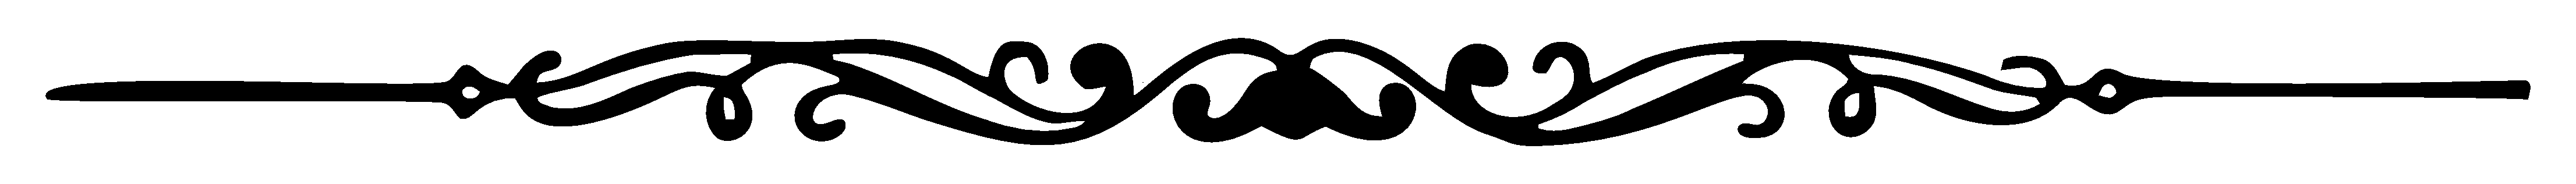
\includegraphics[width=.5\textwidth]{./Vintage-Decorative-Divider.pdf}
 % Vintage-Decorative-Divider.pdf: 0x0 pixel, 300dpi, 0.00x0.00 cm, bb=
\end{center}

\subsection{Rechnen mit Quadratwurzeln}

\begin{regel}[Multiplizieren von Quadratwurzeln]
 Multipliziert man zwei Quadratwurzeln entspricht das dem Produkt der Radikanden unter einer gemeinsamen Quadratwurzel.
 \begin{equation*}
  \sqrt{a}\cdot\sqrt{b} = \sqrt{a\cdot b}
 \end{equation*}
 Das gilt wegen Folgerung \ref{folg:prodpot}, weil:
 \begin{equation*}
  \left(\sqrt{a}\cdot \sqrt{b}\right)^2 = \sqrt{a}^2 \cdot \sqrt{b}^2 = a\cdot b = \left(\sqrt{ab}\right)^2
 \end{equation*}
\end{regel}

\begin{folg}[Quadratwurzel und Quadrat]
Das Quadrat einer Quadratwurzel ist gleich der Quadratwurzel aus dem Quadrat und das ist der Betrag des Radikanden.
\begin{equation*}
 \sqrt{a}^2 =\sqrt{a^2} = |a|
\end{equation*}
Quadrat und Wurzel lassen sich also vertauschen. Ist \(a\geqq 0\), so gilt sogar \(\sqrt{a^2} = a\). Dann kann man davon sprechen, dass sich Quadratwurzel und Quadrat gegenseitig aufheben.
\end{folg}

\begin{regel}[Teilweises Radizieren]
 Lässt sich der Radikand in ein Produkt aus einem Quadrat und einem weiteren Faktor zerlegen, so kann ein Teil des Radikanden radiziert -- also aus der Wurzel herausgezogen -- werden.
 \begin{equation*}
  \sqrt{a^2\cdot b} = \sqrt{a^2} \cdot \sqrt{b} = |a|\cdot\sqrt{b}
 \end{equation*}
\end{regel}

\begin{bsp}
\begin{equation*}
 \sqrt{28} = \sqrt{4\cdot 7} = \sqrt{2^2\cdot 7} = \sqrt{2^2} \cdot \sqrt{7} = 2\sqrt{7}
\end{equation*} 
\end{bsp}

\begin{regel}[Dividieren von Quadratwurzeln]
 Für die Division von Quadratwurzeln gilt die gleiche Regel wie für die Multiplikation: Dividiert man zwei Quadratwurzeln  entspricht das der Quadratwurzel aus dem Quotienten der Radikanden.
 \begin{equation*}
  \frac{\sqrt{a}}{\sqrt{b}} = \sqrt{\frac{a}{b}}
 \end{equation*}
\end{regel}

\begin{folg}[Quadratwurzel aus einer Potenz]
 Ist der Exponent einer Potenz, die unter einer Quadratwurzel steht, gerade, so bewirkt das Radizieren, dass der Exponent halbiert wird.
 \begin{equation*}
  \sqrt{a^{2n}} = \sqrt{\left(a^n\right)^2} = |a^n|
 \end{equation*}
\end{folg}

\begin{bsp}
 \begin{equation*}
  \sqrt{2^6} = \sqrt{\left(2^3\right)^2} = 2^3
 \end{equation*}

\end{bsp}


\begin{regel}[Wurzeln von Wurzeln]
 Steht eine Wurzel unter einer Wurzel, so arbeitet man sich von innen nach außen vor.
 \begin{equation*}
  \sqrt{\sqrt{a^4}}=\sqrt{\sqrt{a^{2\cdot2}}} = \sqrt{\sqrt{\left(a^2\right)^2}} = \sqrt{a^2} = |a|
  \end{equation*}
 Jede der Wurzeln halbiert dabei den Exponenten des Radikanden.
\end{regel}

\begin{regel}[Addieren von Quadratwurzeln]
 Bei der Addition von Quadratwurzeln ist \emph{keine} Vereinfachung möglich!
 \begin{equation*}
  \sqrt{a}+\sqrt{b} \ne \sqrt{a+b}
 \end{equation*}
\end{regel}

\section{Binomische Formeln}
Ein \emph{Binom} ist ein Summenterm, der aus der Summe zweier Größen besteht. Die Binomischen Formeln sind Rechenregeln zur Vereinfachung von Potenzen oder Produkten eines Binoms.

\begin{regel}[Plus-Formel]
 \begin{eqnarray*}
  (a+b)^2 &=& (a+b)\cdot (a+b) = a^2 +ab+ba+b^2\\
  (a+b)^2 &=& a^2+ 2ab +b^2
 \end{eqnarray*}

\end{regel}

\begin{regel}[Minus-Formel]
  \begin{eqnarray*}
  (a-b)^2 &=& (a-b)\cdot (a-b) = a^2 -ab -ba +b^2\\
  (a-b)^2 &=& a^2- 2ab +b^2
 \end{eqnarray*}
\end{regel}

\begin{regel}[Plus-Minus-Formel]
   \begin{eqnarray*}
  (a+b)(a-b) &=& a^2 -ab +ba -b^2\\
  (a+b)(a-b) &=& a^2-b^2
 \end{eqnarray*}
\end{regel}

\begin{regel}[Allgemeine Binomische Formel]
Untersucht man aufeinander folgende Potenzen des Binoms \((a+b)\), so lässt sich nach dem Ausmultiplizieren und dem Zusammenfassen gleichnamiger Terme ein Muster feststellen.
 \begin{eqnarray*}
  (a+b)^0 &=& 1 \\
  (a+b)^1 &=& 1a+1b \\
  (a+b)^2 &=& 1a^2 + 2ab + 1b^2\\
  (a+b)^3 &=& 1a^3 + 3a^2b + 3ab^2 + 1b^3\\
  (a+b)^4 &=& 1a^4 + 4a^3b + 6a^2b^2 + 4ab^3 + 1b^4\\
  (a+b)^5 &=& 1a^5 + 5a^4b + 10 a^3b^2 + 10a^2b^3\\
  && \quad + 5ab^4 + 1b^5
 \end{eqnarray*}
Sortiert man den Summenterm (die rechte Seite) nach der Vielfachheit\footnote{Statt von \emph{Vielfachheit} spricht man hier auch von der \emph{Multiplizität}.} der vorkommenden Variablen, so stellt man fest, dass der erste Summand die erste Variable in der Potenz des Binoms enthält und der Exponent des letzten Summanden ebenso mit dem Exponenten des Binoms übereinstimmt. Bei allen gemischten Produkttermen\footnote{Gemeint sind diejenigen Produktterme, die sowohl \(a\) als auch \(b\) beinhalten} in der Summe entspricht die Summe der Exponenten dem Exponenten des Binoms.
 
Die Zahlen, die hier jeweils an die Terme mit \(a\) und \(b\) multipliziert werden, nennt man die \emph{Binomialkoeffizienten}.\footnote{Ein \emph{Koeffizient} ist eine Zahl, die mit einer Variablen multipliziert wird.} 

Das Muster für die gesamten Terme lässt sich durch die \emph{Allgemeine Binomische Formel} beschreiben.
 \begin{eqnarray*}
  (a+b)^n &=& a^n + \binom{n}{1} a^{n-1}b + \binom{n}{2} a^{n-2}b^2 + \ldots\\&& \quad \ldots + \binom{n}{n-1} ab^{n-1} + b^n\\
  &=& \sum_{k=0}^n \binom{n}{k} a^{n-k}b^k
 \end{eqnarray*}
Dabei steht die Schreibweise \(\binom{n}{k}\) für die \emph{Binomialkoeffizienten}. Diese bestimmt man über folgende Rechenvorschrift:
\begin{equation*}
 \binom{n}{k} = \frac{n!}{k!(n-k)!}
\end{equation*}
Die Binomialkoeffizienten findet man in dieser Abfolge auch im \emph{Pascalschen Dreieck} wieder.
\end{regel}

\begin{beme}[Pascalsches Dreieck]
Die Binomialkoeffizienten \(\binom{n}{k}\) bilden ein recht einfaches Zahlenschema, das das \emph{Pascalsche Dreieck} genannt wird. In diesem Zahlendreieck nummeriert man die Zeilen von 0 beginnend durch. Ebenso werden in jeder Zeile die Zahlen von 0 beginnend nummeriert. Das \(k\)-te Element in der \(n\)-ten Zeile entspricht dann dem Binomialkoeffizienten \(\binom{n}{k}\).

Zum Beispiel ist das 3.~Element in der 5.~Zeile die Zahl \(\binom{5}{3}=\frac{5!}{3!\cdot 2!} = \frac{5\cdot 4}{2\cdot 1} = 10\).

\begin{figure}\begin{center}
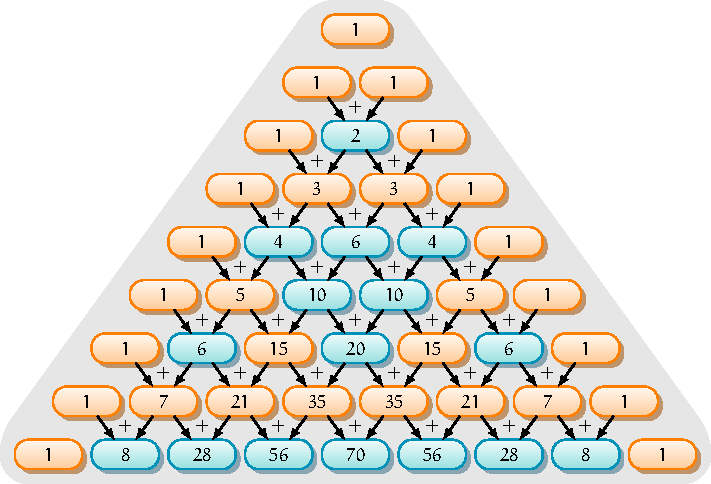
\includegraphics[width=\textwidth]{./pascal_triangle.pdf}
% pascal_triangle.pdf: 0x0 pixel, 300dpi, 0.00x0.00 cm, bb=
\end{center}
\caption{Pascalsches Dreieck}\end{figure}
\end{beme}


\section{Wurzelterme}

\begin{defi}[Wurzelterm]
 Ein Wurzelterm ist ein Term, indem eine Variable oder gesuchte Größe unter einer Wurzel steht.
\end{defi}

\begin{regel}[Definitionsmenge eines Wurzelterms]
 Der Radikand einer Wurzel darf nicht negativ sein. Daraus ergeben sich Bedingungen an die Defintionsmenge der Variablen, die unter Wurzeln stehen.
 
 Zur Bestimmung der Definitionsmenge des Terms \(T(x)=\sqrt{R(x)}\) muss also die Ungleichung \(R(x)\geqq 0\) gelöst werden.
\end{regel}

\begin{bsp}[Bestimmung der Definitionsmenge]
 \begin{eqnarray*}
  T(x) &=& \sqrt{1-x}\\
  1-x &\geqq& 0 \\
  1 &\geqq & x \\
  \mathcal{D}_T &=& ]-\infty ; 1]
 \end{eqnarray*}

\end{bsp}


\begin{regel}[Rationalmachen eines Nenners]
 Bei einem Term, der nach der gesuchten Größe aufgelöst werden soll, ist einer der nötigen Schritte, Wurzeln aus einem oder mehreren Nennern zu entfernen. Das kann durch geschicktes Erweitern des jeweiligen Bruchs erreicht werden.
 
 Fall~1: Der Nenner eines Terms besteht aus einer Wurzel.
 
 Dann erweitert man den Bruch mit dem Nenner.
 \begin{equation*}
  \frac{a}{\sqrt{R}} = \frac{a\cdot \sqrt{R}}{\sqrt{R}\cdot\sqrt{R}} = \frac{a\sqrt{R}}{R} 
 \end{equation*}
 
 Fall~2: Im Nenner steht eine Wurzel in einer Summe oder Differenz.
 
 Hier nutzt man die dritte Binomische Formel (Plus-Minus-Formel), um die Wurzel aus dem Nenner zu eliminieren.
 \begin{eqnarray*}
  \frac{a}{b+\sqrt{R}} &=& \frac{a\cdot \left(b-\sqrt{R}\right)}{\left(b+\sqrt{R}\right)\cdot \left(b-\sqrt{R}\right)} = \frac{a\left(b-\sqrt{R}\right)}{b^2-R}\\
  \frac{a}{b-\sqrt{R}} &=& \frac{a\cdot \left(b+\sqrt{R}\right)}{\left(b-\sqrt{R}\right)\cdot \left(b+\sqrt{R}\right)} = \frac{a\left(b+\sqrt{R}\right)}{b^2-R}
 \end{eqnarray*}
 Nach dem Erweitern ist es meist sinnvoll das Produkt im Zähler so stehen zu lassen und \emph{nicht} auszumultiplizieren.
\end{regel}

\begin{bsp}[Rationalmachen des Nenners, Fall~1]
 \begin{eqnarray*}
  \frac{2}{\sqrt{x+1}} &=& \frac{2\sqrt{x+1}}{x+1}
 \end{eqnarray*}
\end{bsp}
\begin{bsp}[Rationalmachen des Nenners, Fall~2]
 \begin{eqnarray*}
  \frac{2}{x+\sqrt{x+1}} &=& \frac{2\cdot \left(x-\sqrt{x+1}\right)}{\left(x+\sqrt{x+1}\right)\cdot \left(x-\sqrt{x+1}\right)} \\ &=& \frac{2\left(x-\sqrt{x+1}\right)}{x^2-(x+1)}
 \end{eqnarray*}
\end{bsp}

\section{n-te Wurzel}

\begin{defi}[n-te Wurzel]
 Die Lösungen der Gleichung \(x^n=a\) nennt man die \(n\)-ten Wurzeln von \(a\). Kurz:
 \begin{eqnarray*}
  x^n &=& a \\
  x &=& (\pm)\sqrt[n]{a}
 \end{eqnarray*}
 Eine negative Lösung tritt dabei nur dann auf, wenn entweder \(n\) gerade ist oder \(n\) ungerade und \(a\) negativ sind. In letzterem Fall gibt es keine positive Lösung.
 Für gerades \(n\) gibt es immer zwei reelle Lösungen, für ungerades \(n\) stets nur eine.
\end{defi}

\begin{bsp}
 \begin{eqnarray*}
  x^3 &=& -27 \\
  x &=& \sqrt[3]{-27} = -3
 \end{eqnarray*}
 \begin{eqnarray*}
  x^4 &=& 81 \\
  x &=& \pm \sqrt[4]{81} = \pm 3
 \end{eqnarray*}
 \begin{eqnarray*}
  x^5 &=& 32 \\
  x&=& \sqrt[5]{32} = \sqrt[5]{2^5} = 2
 \end{eqnarray*}

\end{bsp}

\begin{regel}[Stammbruch als Exponent]
 Die \(n\)-te Wurzel entspricht der Umkehrung der \(n\)-ten Potenz. Es gilt:
 \Large
 \begin{equation*}
  \sqrt[n]{x^n} = x = x^1 = x^{\frac{n}{n}} = x^{n\cdot \frac{1}{n}} = \left(x^n\right)^{\frac{1}{n}}
 \end{equation*}
 \normalsize
 Oder allgemeiner für \(a\in\mathbb{R}^+\) und \(n\in\mathbb{N}\):
 \Large
 \begin{equation*}
  \sqrt[n]{a} = a^{\frac{1}{n}}
 \end{equation*}\normalsize
 Die \(n\)-te Wurzel ist also nichts anderes als die \(\frac{1}{n}\)-te Potenz.
\end{regel}

\begin{regel}[Rationale Exponenten]
 Die \(n\)-te Wurzel aus der \(m\)-ten Potenz kann einfach als eine Potenz geschrieben werden. Sie hat dann den Exponenten \(\frac{m}{n}\).
 \begin{equation*}
  \sqrt[n]{a^m} = \left(a^m\right)^{\frac{1}{n}} = a^{m\cdot \frac{1}{n}} = a^{\frac{m}{n}}
 \end{equation*}
 Generell ist dieser Ausdruck nur für \(a\geqq 0\) definiert. Ob auch negative Werte für \(a\) möglicherweise zugelassen werden können, hängt davon ab, ob \(m\) oder \(n\) gerade oder ungerade sind.
\end{regel}

\begin{beme}
 Auch für rationale Zahlen als Exponent gelten weiter die \nameref{sec:potenzgesetze}. Also gilt:
 \begin{eqnarray*}
  a^{\frac{m}{n}} \cdot a^{\frac{p}{q}} &=& a^{\frac{m}{n}+\frac{p}{q}} = a^{\frac{mq+pn}{nq}}\\
  a^{\frac{m}{n}} \div a^{\frac{p}{q}} &=& a^{\frac{m}{n}-\frac{p}{q}} = a^{\frac{mq-pn}{nq}}\\
  \left(a^{\frac{m}{n}}\right)^{\frac{p}{q}} &=& a^{\frac{m}{n}\cdot \frac{p}{q}} = a^{\frac{mp}{nq}} \\
  a^{\frac{m}{n}} \cdot b^{\frac{m}{n}} &=& (ab)^{\frac{m}{n}}\\
  a^{\frac{m}{n}} \div b^{\frac{m}{n}} &=& \left(\frac{a}{b}\right)^{\frac{m}{n}}
 \end{eqnarray*}

\end{beme}


\section{Quadratische Terme}
\label{sec:quadterm}

\begin{defi}[Quadratischer Term]
 Ein Term \(T(x)\) heißt \emph{quadratisch}, wenn in ihm nur Summanden ohne Variable oder mit Variable in erster Potenz  oder mit Variable im Quadrat vorkommen. Ein quadratischer Term ist zum Beispiel:
 \begin{equation*}
  T(x) = 2x^2-3x+1+x^2+5x
 \end{equation*}
Fasst man in einem quadratischen Term alle gleichnamigen Terme zusammen, so erhält man nur noch drei Summanden: der erste Summand enthält \(x^2\) und danach folgt ein linearer Term.
 \begin{equation*}
  T(x) = 2x^2-3x+1+x^2+5x = 3x^2 +2x+1
 \end{equation*}
 Daraus ergibt sich die allgemeine Form für einen linearen Term:
 \begin{equation*}
  T(x) = ax^2+bx+c
 \end{equation*}
 Diese Schreibweise nennt man auch die \emph{Normalform} eines quadratischen Terms.
\end{defi}

\subsection{Quadratische Funktion}
\begin{figure}
\centering
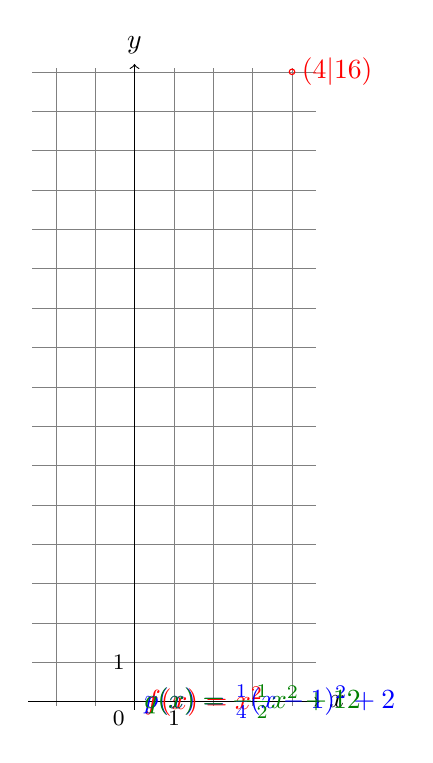
\begin{tikzpicture}[domain=-2.6:4.6,y=1cm,x=1cm,scale=0.5]
    \draw[very thin,color=gray] (-2.6,-0.1) grid (4.6,16.1);
    \draw[->] (-2.7,0) -- (4.7,0) node[right] {$x$};
    \draw[->] (0,-0.2) -- (0,16.2) node[above] {$y$};
    \draw (0,0) node [anchor=north east] {\footnotesize \(0\)};
    \draw (1,0) node [anchor=north] {\footnotesize  \(1\)};
    \draw (0,1) node [anchor=east] {\footnotesize \(1\)};
    \draw[color=red] plot[id=x2] function{x*x} 
        node[right] {$f(x) =x^2$};
    \draw[color=red] (4,16) circle (2pt) node[anchor=west] {\((4|16)\)};
    \draw[color=blue] plot[id=bx2] function{0.25*(x-1)**2 +2} 
        node[right] {$p(x) =\frac{1}{4}(x-1)^2+2$};
    \draw[color=green!50!black] plot[id=cx2] function{-0.5*x**2 +12} 
        node[right] {$q(x) =-\frac{1}{2}x^2+12$};   
\end{tikzpicture}
\caption{Parabeln - Graphen quad. Funktionen}
\end{figure}

\begin{beme}
Der Graph einer quadratischen Funktion, also einer Funktion mit quadratischem Term, ist eine \emph{Parabel}.
Der Funktionsgraph \emph{Parabel} ist eindeutig bestimmt durch den \emph{Scheitelpunkt} und die \emph{Öffnungsweite} und \emph{Öffnungsrichtung}.

Die Parabel, die zum einfachsten quadratischen Term \(f(x)=x^2\) gehört, nennt man die \emph{Normalparabel}.

Ist die Funktion in der Form
\begin{equation*}
 f(x) = ax^2+bx+c
\end{equation*}
gegeben, so kann man anhand des Koeffizienten \(a\) Öffnungsweite und Öffnungsrichtung der Parabel ablesen:
\begin{itemize}
 \item Gilt \(|a|>1\), dann ist die Parabel schmaler als die Normalparabel.
 \item Gilt \(|a|<1\), dann ist die Parabel weiter als die Normalparabel.
 \item Gilt \(a>0\), dann ist die Parabel nach oben geöffnet. Der Scheitelpunkt ist der tiefste Punkt (Minimum) der Parabel.
 \item Gilt \(a<0\), dann ist die Parabel nach unten geöffnet. Der Scheitelpunkt ist der höchste Punkt (Maximum) der Parabel.
\end{itemize}

Am Parameter \(c\) kann man ablesen, bei welchem Wert die \(y\)-Achse von der Parabel geschnitten wird, denn \(f(0)=c\).

\end{beme}

\subsection{Scheitelpunktsform}

\begin{beme}
 Der Scheitelpunkt kann in der Normalform eines quadratischen Terms nicht direkt abgelesen werden. Um das zu erreichen, verwandelt man den Term in die \emph{Scheitelpunktsform} durch die \emph{quadratische Ergänzung}.
 
\end{beme}

\begin{regel}[Quadratische Ergänzung]
 Bei der Quadratischen Ergänzung versucht man den Term in eine Summe aus einem quadrierten Binom und einer Zahl umzuformen.
 Dazu wird passend eine \emph{kreative Null} eingefügt. Das bedeutet, dass man eine Zahl addiert und gleich wieder subtrahiert. Dadurch ändert sich der Wert des Terms nicht.
 
 \begin{align*}
  ax^2+bx+c &= a\left(x^2+\frac{b}{a}x\right) +c \\
  &= a\left(x^2+\frac{b}{a}x + \underbrace{\left(\frac{b}{2a}\right)^2 - \left(\frac{b}{2a}\right)^2}_{=0} \right) + c \\
  &= a\left(\left(x+\frac{b}{2a}\right)^2 - \left(\frac{b}{2a}\right)^2 \right) +c \\
  &= a\left(x+\underbrace{\frac{b}{2a}}_{-x_S}\right)^2 + \underbrace {c - \frac{b^2}{4a}}_{y_S} \\
  &= a\left(x-x_S\right)^2 + y_S
 \end{align*}

 Für die Koordinaten des Scheitelpunkts \(S\) gilt also:
 \begin{align*}
  x_S &= -\frac{b}{2a} \\
  y_S &= c - \frac{b^2}{4a}
 \end{align*}
 Es gilt \(f(x_S) = \underbrace{a\left(x_S-x_S\right)^2}_{=0} + y_S = y_S\).
\end{regel}

\begin{bsp}[Ablesen des Scheitelpunkts]
 Der Graph der quadratischen Funktion 
 \begin{equation*}
  p(x) = \frac{1}{10} (x\underbrace{+5}_{-x_S})^2 \underbrace{+20}_{y_S}
 \end{equation*}
 hat seinen Scheitelpunkt bei \(S (-5\mid 20)\).
\end{bsp}


\begin{bsp}
 Gegeben sei \(f(x)=\frac{1}{2}x^2-2x+5\).
 
 Umwandlung in die Scheitelpunktsform durch quad. Ergänzung: 
 \begin{align*}
  \frac{1}{2}x^2 -2x +5 &= \frac{1}{2}\left(x^2 -4x \right) +5 \\
  &= \frac{1}{2} \left(\underbrace{x^2 -4x + 2^2}_{\text{binom. Formel}} -2^2\right) +5 \\
  &= \frac{1}{2} \left((x-2)^2 -4\right) +5 \\
  &= \frac{1}{2} (x-2)^2 -2 +5 \\
  &= \frac{1}{2} (x-2)^2 +3 \\
  x_S &= +2 \\
  y_S &= +3
 \end{align*}

 Somit liegt hier der Scheitelpunkt bei \(S(2|3)\). Die Parabel ist weiter als die Normalparabel und nach oben geöffnet. Sie schneidet die \(y\)-Achse bei \(y=5\).
\end{bsp}

\begin{beme}[Nullstellen]
 Die Schnittpunkte eines Graphen mit der \(x\)-Achse nennt man seine \emph{Nullstellen}. Eine Parabel kann bis zu zwei Nullstellen haben, da quadratische Gleichungen bis zu zwei Lösungen haben können. Die Bestimmung der Nullstellen entspricht der Lösung der quadratischen Gleichung \(ax^2+bx+c =0\).
\end{beme}

\begin{defi}{Quadratische Gleichung}
 Eine \emph{quadratische Gleichung} liegt vor, wenn die höchste Potenz einer Variablen in der Gleichung ihr Quadrat ist. Quadratische Gleichungen können mehr als eine Lösung besitzen.
 
 Gleichungen wie
 \begin{align*}
  x^2 &= 1 & \mathcal{L}&=\lbrace -1; +1\rbrace\\
  (x+1)^2 &= 0 & \mathcal{L} &= \lbrace -1 \rbrace \\
  x^2 &= -5 & \mathcal{L}&= \lbrace \,\rbrace \\
  2x^2+4x-1 &= 0 & \mathcal{L} &= \left\lbrace -1+\frac{\sqrt{6}}{2}; -1-\frac{\sqrt{6}}{2}\right\rbrace \\
  (x-1)^2+5 &= 10 & \mathcal{L} &= \left\lbrace 1+\sqrt{5};1-\sqrt{5}\right\rbrace   
 \end{align*}
 sind quadratische Gleichungen.
\end{defi}

\begin{regel}
 Befindet sich in einer quadratischen Gleichung auf der einen Seite des Gleichheitszeichens ein Term in Scheitelpunktsform und auf der anderen Seite eine Zahl, so lässt sich diese Gleichung mit wenigen Äquivalenzumformungen lösen.
 
 Zu beachten ist hierbei, dass das Anwenden der Quadratwurzel auf eine Gleichung zur Folge hat, dass in der nächsten Zeile positive und negative Werte möglich sind.
 \begin{align*}
  x^2 &= a &&|\sqrt{\ldots}\\
  \sqrt{x^2} = |x| &= \sqrt{a} \\
  x &= \pm \sqrt{a}
 \end{align*}
 Denn:
 \begin{align*}
  \sqrt{a}^2 &= a & \left(-\sqrt{a}\right)^2 = a 
 \end{align*}

\end{regel}

\begin{bsp}[Quadratische Gleichung lösen]
 \begin{align*}
  4(x-2)^2 +3&= 11 && | -3\\
  4(x-2)^2 &= 8 && | \div 4\\
  (x-2)^2 &= 2 && | \sqrt{\ldots} \\
  x-2 &= \pm \sqrt{2} && | +2 \\
  x &= 2 \pm \sqrt{2} \\
  \mathcal{L} &= \lbrace 2-\sqrt{2}; 2+\sqrt{2}\rbrace
 \end{align*}
 Hier verkompliziert ein Ausmultiplizieren von \((x-2)^2\) eher den Weg zur Lösung der Gleichung.
\end{bsp}

Doch auch, wenn der quadratische Term \emph{nicht} in der Scheitelpunktsform vorliegt, gibt es eine einfach anwendbare Regel zur Bestimmung der Lösungen. Da diese Regel von so großer Bedeutung für die Lösung von Gleichungen ist, nennt man sie auch die \emph{Mitternachtsformel}. (Wird man mitten in der Nacht geweckt, sollte man diese Formel aufsagen können.)

\begin{ssatz}[Mitternachtsformel / Lösungsformel]
 Eine quadratische Gleichung der Form
 \begin{equation*}
  ax^2+bx+c =0
 \end{equation*}
 hat die Lösung(en)
 \begin{blockwhitebox}
 \begin{equation*}  x_{1/2} = \frac{-b\pm \sqrt{b^2-4ac}}{2a} 
 \end{equation*}
 \end{blockwhitebox}
 wenn \(D = b^2-4ac \geqq 0\).

\end{ssatz}

\begin{bew}
 Der Nachweis erfolgt über die quadratische Ergänzung.
 \begin{align*}
  ax^2+bx+c &= 0 \\
  \text{quadratische Ergänzung} & \\
 a\left(x+\frac{b}{2a}\right)^2 + c - \frac{b^2}{4a} &= 0 \\
  a\left(x+\frac{b}{2a}\right)^2 &= \frac{b^2}{4a} -c \\
  a\left(x+\frac{b}{2a}\right)^2 &= \frac{b^2-4ac}{4a} \\
  \left(x+\frac{b}{2a}\right)^2 &= \frac{b^2-4ac}{4a^2} \\
  x_{1/2} + \frac{b}{2a} &= \pm \sqrt{\frac{b^2-4ac}{4a^2}} \\
  x_{1/2} &= -\frac{b}{2a} \pm \frac{\sqrt{b^2-4ac}}{2a} \\
  x_{1/2} &= \frac{-b\pm \sqrt{b^2-4ac}}{2a} 
 \end{align*}

\end{bew}

\begin{regel}[Diskriminante]
 An der \emph{Diskriminante} \(D = b^2-4ac\) kann man ablesen, wie viele Lösungen eine quadratische Gleichung besitzt.
 
 \begin{itemize}
  \item \(D>0\): Die Gleichung hat zwei Lösungen.
  \item \(D=0\): Die Gleichung hat genau eine Lösung.
  \item \(D<0\): Die Gleichung ist in den reellen Zahlen nicht lösbar.
 \end{itemize}
\end{regel}

\subsection{Gemeinsame Punkte von Funktionsgraphen}

In Anwendungen ist es häufig nötig die Existenz oder die genaue Lage gemeinsamer Punkte von Funktionsgraphen zu bestimmen. Dazu gibt es zwei verschiedene Herangehensweise, die zum gleichen mathematischen Problem führen. Im Folgenden werden diese Strategien anhand der Funktionen \(g(x)=\frac{1}{2}x+1\) und \(f(x)=(x-2)^2-1\) vorgestellt.

\begin{figure}
 \begin{center}
   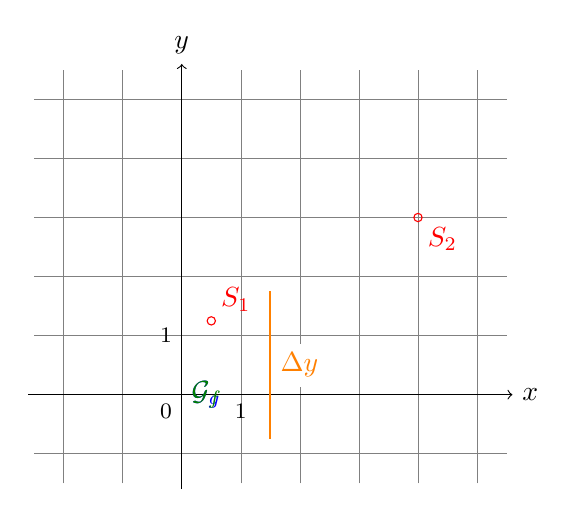
\begin{tikzpicture}[domain=-2.5:5.5,y=1cm,x=1cm,scale=0.75]
    \draw[very thin,color=gray] (-2.5,-1.5) grid (5.5,5.5);
%     \draw[very thin,color=gray, xstep=pi/8, ystep=0.25] (0,0) grid (pi/2,1);
    \draw[->] (-2.6,0) -- (5.6,0) node[right] {$x$};
    \draw[->] (0,-1.6) -- (0,5.6) node[above] {$y$};

    \draw (0,0) node [anchor=north east] {\footnotesize \(0\)};
    \draw (1,0) node [anchor=north] {\footnotesize  \(1\)};
    \draw (0,1) node [anchor=east] {\footnotesize \(1\)};
%     \clip (-1.6,-2.3) rectangle (7.1,2.3);
     \draw[color=blue] plot[id=spger, domain=-2.5:5.5] function{0.5*x+1} node[right] {$\mathcal{G}_g$};
     \draw[color=green!50!black] plot[id=sppar, domain=-0.6:4.6, samples=200] function{(x-2)**2-1} node[right] {$\mathcal{G}_f$};
    \draw[red] (0.5,1.25) circle (2pt) node[anchor=south west]{\(S_1\)};
    \draw[red] (4,3) circle (2pt) node[anchor=north west]{\(S_2\)};
    
    \draw[thick, orange] (1.5,-0.75) -- node[anchor=west, fill=white]{\(\Delta y\)} (1.5,1.75); 
%     \draw[color=red] node[right] {$f(x) =\sin(x)$};
%     \draw[color=red] (4,16) circle (2pt) node[anchor=west] {\((4|16)\)};
%     \draw[color=blue] plot[id=cosx, samples=200] function{cos(x)} 
%         node[right] {$\cos(\alpha)$};
%     \draw[color=green!50!black] plot[id=tanx, domain=(-pi/2+0.1):(pi/2-0.1), samples=200] function{tan(x)}; 
%     \draw[color=green!50!black] plot[id=tan2x,  domain=(pi/2+0.1):(3*pi/2-0.1), samples=200] function{tan(x)};
%     \draw[color=green!50!black] (4.4,1.5) node[right,fill=white] {$\tan(\alpha)$};   
\end{tikzpicture}
 \end{center}
\caption{Schnittpunkte der Geraden \(g(x)=\frac{1}{2}x+1\) mit der Parabel \(f(x)=(x-2)^2-1\)}
\end{figure}

Der Graph der Funktion \(f(x)=(x-2)^2-1\) ist die Menge aller Punkte, die die Funktionsgleichung erfüllen. Es gilt:
\begin{equation*}
 \mathcal{G}_f = \left\lbrace P(x|y) \mid y=(x-2)^2-1 \right\rbrace
\end{equation*}
Gleiches gilt für die Funktion \(g(x)=\frac{1}{2}x+1\).
\begin{equation*}
 \mathcal{G}_g = \left\lbrace P(x|y) \mid y=\frac{1}{2}x+1 \right\rbrace
\end{equation*}
Die gemeinsamen Punkte der Funktionsgraphen sind also genau diejenigen, die in diesen beiden Mengen enthalten sind. Für einen gemeinsamen Punkt \(S\) gilt daher:
\begin{equation*}
 \mathcal{G}_f \ni S(x|y) \in \mathcal{G}_g
\end{equation*}
Das bedeutet, dass für den gleichen Wert von \(x\) beide Funktionsterme den gleichen \(y\)-Wert ergeben müssen.

\begin{regel}[Gleichsetzen der Funktionsterme]
 Bei gemeinsamen Punkten zweier Funktionsgraphen müssen deren Funktionsterme an der jeweiligen Stelle den gleichen Wert ergeben. Um diese Punkte zu bestimmen, genügt es die Funktionterme gleichzusetzen und die Gleichung zu lösen.
 
 Zur Bestimmung gemeinsamer Punkte der Graphen \(\mathcal{G}_f\) und \(\mathcal{G}_g\):
 \begin{blockwhitebox}
  \begin{equation*}
   f(x) = g(x)
  \end{equation*}
 \end{blockwhitebox}
 Die Lösungsmenge dieser Gleichung beinhaltet die \(x\)-Koordinaten \emph{aller} gemeinsamen Punkte. Die zugehörigen \(y\)-Koordinaten werden anschließend durch Auswertung eines der beiden Funktionsterme für die entsprechenden Werte von \(x\) bestimmt.
\end{regel}

\begin{bsp}
Berechnung der \(x\)-Koordinaten der gemeinsamen Punkte:
 \begin{align*}
  (x-2)^2 -1 &= \frac{1}{2}x+1 && \\
  x^2-4x+4-1 &= \frac{1}{2}x+1 &&| -1-\frac{1}{2}x\\
  x^2-4.5x+2 &= 0 \\\intertext{Lösungsformel:}
  x_{1/2} &= \frac{4.5\pm \sqrt{4.5^2-8}}{2} \\
  &= \frac{4.5\pm\sqrt{12.25}}{2} \\
  & = \left\lbrace\begin{array}{c}
                                                 4 \\ \frac{1}{2}
                                                \end{array}\right.
 \end{align*}
 Zur Bestimmung der \(y\)-Koordinaten ist es egal, welchen der Funktionsterme man benutzt.
 \begin{align*}
  f(4)&=(4-2)^2-1 & g(4) &= \frac{1}{2}\cdot 4+1\\
      &=4-1=3 & &=3\\
  f\left(\frac{1}{2}\right) &= \left(\frac{1}{2}-2\right)^2-1 & g\left(\frac{1}{2}\right) &= \frac{1}{2}\cdot\frac{1}{2}+1\\
  &= 2\frac{1}{4} -1 = 1\frac{1}{4}& &= 1\frac{1}{4} 
 \end{align*}

\end{bsp}

\begin{bsp}[Parameter bestimmen]
 Bestimme die Werte von \(m\), für die die Graphen der Funktionen
 \begin{align*}
  p(x) &= -(x-2)^2+1 &&\text{und}&
  g(x) &= mx + 1
 \end{align*}
 gemeinsame Punkte besitzen.
 
 Die \(x\)-Koordinaten der potenziellen Schnittpunkte werden über das Gleichsetzen der Funktionsterme bestimmt:
 \begin{align*}
  -(x-2)^2+1 &= mx +1\\
  -(x^2-4x+4) &= mx \\
  -x^2+4x-mx-4 &= 0 \\
  -x^2+(4-m)x -4 &= 0\\
  \intertext{Anwenden der Lösungsformel:}
  x_{1/2} &= \frac{-(4-m)\pm\sqrt{(4-m)^2-4\cdot 4}}{-2} 
 \end{align*}
 
 Die Gleichung hat nur dann Lösungen, wenn die Diskriminante \(D=(4-m)^2-16\) größer oder gleich null ist.
 \begin{align*}
  D=(4-m)^2-16&\geq 0&&|+16\\
    (4-m)^2 &\geq +16 &&|\sqrt{\ldots}\\
    4-m &\geq +4 & &\text{oder} & 4-m&\leq -4 \\
    -m &\geq 0 & &\text{oder} & -m&\leq -8 \\
    m &\leq 0 & &\text{oder} & m&\geq 8
 \end{align*}
 
 Für alle \(m\leq 0 \) und für alle \(m\geq 8\) haben die Graphen der beiden Funktionen Schnittpunkte.
 \begin{figure}
 \begin{center}
   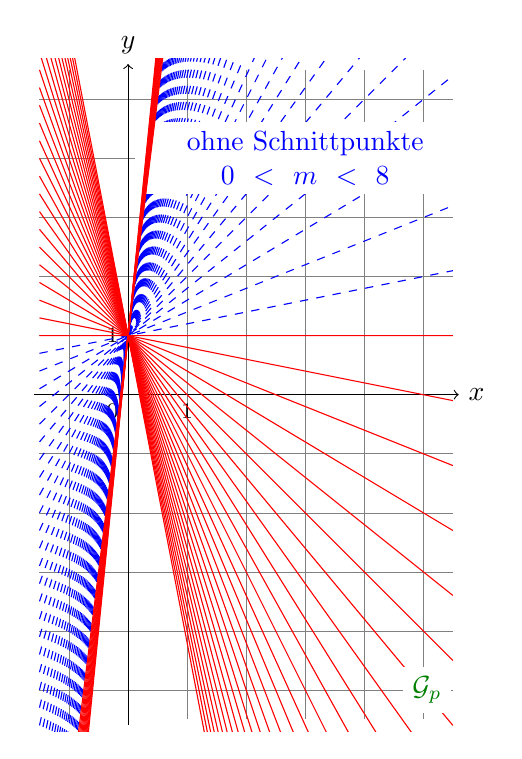
\begin{tikzpicture}[domain=-1.5:5.5,y=1cm,x=1cm,scale=0.75]
   
    \draw[very thin,color=gray] (-1.5,-5.5) grid (5.5,5.5);
%     \draw[very thin,color=gray, xstep=pi/8, ystep=0.25] (0,0) grid (pi/2,1);
    \draw[->] (-1.6,0) -- (5.6,0) node[right] {$x$};
    \draw[->] (0,-5.6) -- (0,5.6) node[above] {$y$};
 
    \draw (0,0) node [anchor=north east] {\footnotesize \(0\)};
    \draw (1,0) node [anchor=north] {\footnotesize  \(1\)};
    \draw (0,1) node [anchor=east] {\footnotesize \(1\)};
    \clip (-1.7,-5.7) rectangle (5.7,5.7);
    \foreach \m in {0.2,0.4,...,7.8}{
     \draw[color=blue, dashed] plot[variable=\x,domain=-1.5:5.5] ({\x},{\m*\x+1});};
     \draw[blue](3,4) node[fill=white,anchor=center,text width=4.1cm, align=center]{ohne Schnittpunkte\\ $0<m<8$};
     
     \foreach \m in {-5.2,-5,...,0}{
     \draw[color=red] plot[variable=\x,domain=-1.5:5.5] ({\x},{\m*\x+1});};
     \foreach \m in {8,8.2,...,10}{
     \draw[color=red] plot[variable=\x,domain=-1.5:5.5] ({\x},{\m*\x+1});};
     \draw[color=green!50!black,thick] plot[id=sppar2, domain=-1.5:4.8, samples=200] function{-(x-2)**2+1};
     \draw[color=green!50!black] (4.65,-5) node[right,fill=white] {$\mathcal{G}_p$};
%     \draw[red] (0.5,1.25) circle (2pt) node[anchor=south west]{\(S_1\)};
%     \draw[red] (4,3) circle (2pt) node[anchor=north west]{\(S_2\)};
  
\end{tikzpicture}
 \end{center}
\caption{Schnittpunkte der Geraden aus der Geradenschar \(g(x)=mx+1\) mit der Parabel \(f(x)=-(x-2)^2+1\)}
\end{figure}

\end{bsp}


\begin{regel}[Nullstellen der Differenz]
 Eine andere Sichtweise führt ebenso zur Bestimmung der gemeinsamen Punkte: Zu jedem Wert der Variable \(x\) liefern beide Funktionsterme einen eigenen Wert \(y\). Wenn sich diese Werte nicht voneinander unterscheiden, wenn also die Differenz \(\Delta y\) der Funktionswerte gleich 0 ist, so handelt es sich um einen gemeinsamen Punkt der Funktionsgraphen.
 \begin{align*}
  \Delta y = y_f -y_g &\stackrel{!}{=} 0\\
  f(x)-g(x) &= 0 \\
  \intertext{in unserem Beispiel:}
  (x-2)^2-1-\left(\frac{1}{2}x+1\right) &=0
 \end{align*}
 Die weitere Rechnung verläuft dann wie vorher.
\end{regel}

Die Bestimmung gemeinsamer Punkte führt nicht nur bei Parabel und Gerade zu einer quadratischen Gleichung. Auch bei Parabel--Parabel, Hyperbel--Gerade und Hyperbel--Hyperbel kann oft dieses Problem darauf zurückgeführt werden, eine quadratische Gleichung lösen zu müssen.

\begin{bsp}
 Bestimme die gemeinsamen Punkte der Graphen der Funktionen \(f(x) =\frac{4}{x-2}+1\) und \(g(x)=2x-1\).
 
 \begin{figure}
  \begin{center}
      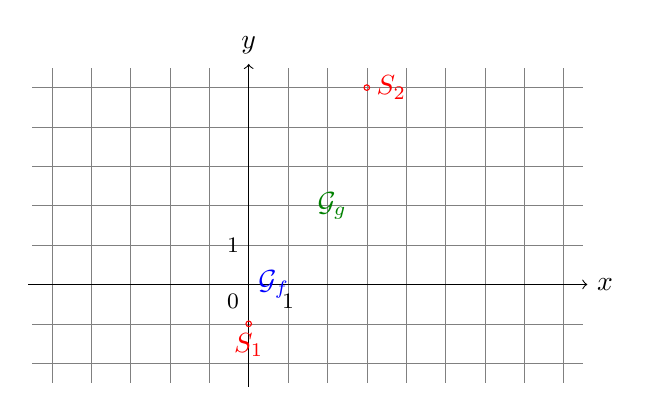
\begin{tikzpicture}[domain=-5.5:8.5,y=1cm,x=1cm,scale=0.5]
    \draw[very thin,color=gray] (-5.5,-2.5) grid (8.5,5.5);
%     \draw[very thin,color=gray, xstep=pi/8, ystep=0.25] (0,0) grid (pi/2,1);
    \draw[->] (-5.6,0) -- (8.6,0) node[right] {$x$};
    \draw[->] (0,-2.6) -- (0,5.6) node[above] {$y$};

    \draw (0,0) node [anchor=north east] {\footnotesize \(0\)};
    \draw (1,0) node [anchor=north] {\footnotesize  \(1\)};
    \draw (0,1) node [anchor=east] {\footnotesize \(1\)};
    \clip (-5.6,-2.6) rectangle (10,5.6);
     \draw[color=blue] plot[id=sphyp1, domain=2.05:8.5, samples=200] function{4/(x-2)+1} node[right] {$\mathcal{G}_f$};
     \draw[color=blue] plot[id=sphyp2, domain=-5.5:1.95, samples=200] function{4/(x-2)+1};
     \draw[color=green!50!black] plot[id=spger2, domain=-2:4] function{2*x-1} ;
    \draw[color=green!50!black] (1.5,2) node[right] {$\mathcal{G}_g$};
    \draw[red] (0,-1) circle (2pt) node[anchor=north]{\(S_1\)};
    \draw[red] (3,5) circle (2pt) node[anchor=west]{\(S_2\)}; 
\end{tikzpicture}
  \end{center}
 \caption{Gemeinsame Punkte von Gerade \(2x-1\) und Hyperbel \(\frac{4}{x-2}+1\).}
 \end{figure}
  Gleichsetzen der Funktionsterme:
 \begin{align*}
  f(x) &= g(x) \\
  \frac{4}{x-2}+1 &= 2x-1 && |-1\\
  \frac{4}{x-2} &= 2x-2 &&|\cdot (x-2) \\
  4 &= (2x-2)(x-2) \\
  4 &= 2x^2 -4x-2x+4 && |-4 \\
  0 &= 2x^2-6x \\
  \intertext{Faktorisieren:}
  0&= 2x\cdot (x-3) \\
  \intertext{Ein Produkt ist 0, wenn einer der Faktoren 0 ist.}
  x_1 &= 0& x_2=+3
 \end{align*}
 Darauf folgt die Bestimmung der \(y\)-Koordinaten der Schnittpunkte:
 \begin{align*}
  g(x_1) = g(0) &= 2\cdot 0 -1 = -1 \\
  g(x_2) = g(3) &= 2\cdot 3 -1 = 5
 \end{align*}
 Die Schnittpunkte sind also \(S_1 (0|-1)\) und \(S_2 (3|5)\).
\end{bsp}

\section{Lineare Gleichungssysteme (\ensuremath{3\times 3})}

In der 8.~Jahrgangsstufe wurden bereits Systeme aus zwei Gleichungen mit zwei Unbekannten behandelt (\(2\times2\)). Dieses Konzept wird jetzt um eine Variable und Gleichung erweitert (\(3\times 3\)).
Die Lösungsverfahren bleiben dabei prinzipiell die gleichen. Lediglich die Anzahl der Schritte bis zur Lösung ist höher. Dem Leser sollten bereits das Einsetzungsverfahren und das Additionsverfahren zur Lösung von \(2\times 2\)-Gleichungssystemen bekannt sein.

Ein \(3\times 3\)-Gleichungssystem hat folgende Form:
\begin{align*}
 a_1 x + b_1 y + c_1 z &= d_1 \\
 a_2 x + b_2 y + c_2 z &= d_2 \\
 a_3 x + b_3 y + c_3 z &= d_3
\end{align*}
mit \(a_i, b_i, c_i, d_i \in\mathbb{R}\) für \(i\in\lbrace 1;2;3\rbrace\).

Die Lösung eines solchen Gleichungssystems besteht, wenn sie eindeutig ist, aus einem Zahlentripel \((x,y,z)\).

\begin{defi}
 Ein Gleichungssystem mit mehr Gleichungen als Variablen heißt \emph{überbestimmt}. Ein Gleichungssystem mit weniger Gleichungen als Variablen nennt man \emph{unterbestimmt}.
\end{defi}

\begin{regel}[Einsetzungsverfahren]
 
\end{regel}

\begin{bsp}[Einsetzungsverfahren]
  \begin{align*}
  \text{I} && x+y-z &= 2\\
  \text{II} && 3x+2y+z &= 8\\
  \text{III} && x+y+z &= 4
 \end{align*}
 Auflösen von I nach \(x\):
 \begin{align*}
  \text{I'} && x&= 2-y+z
 \end{align*}
 Einsetzen in II und Auflösen nach \(y\):
 \begin{align*}
  \text{II} && 3x+2y+z &= 8\\
  &&3(2-y+z)+2y+z &= 8 \\
  &&6-3y+3z+2y+z &= 8 \\
  &&  -y+4z &= 2 \\
  \text{II'}&&  y &= 4z-2
 \end{align*}
 Einsetzen in III und Auflösen nach \(z\):
 \begin{align*}
  \text{III} && x+y+z &= 4 \\
             && (2-y+z) + y +z &= 4\\
             && (2-(4z-2) +z) +(4z-2) +z &= 4\\
             && 2+2z &= 4 \\
             && z&=1
 \end{align*}
 Rückeinsetzen in II' und I':
 \begin{align*}
  \text{II'}&&  y &= 4z-2 = 2\\
  \text{I'} && x &= 2-y+z = 1
 \end{align*}
 Angabe der Lösungsmenge:
 \begin{equation*}
  \mathcal{L} = \left\lbrace (1;2;1) \right\rbrace
 \end{equation*}
\end{bsp}

\begin{bsp}[modifiziertes Einsetzungsverfahren]
 \begin{align*}
  \text{I} && x+y-z &= 2\\
  \text{II} && 3x+2y+z &= 8\\
  \text{III} && x+y+z &= 4
 \end{align*}
 Lösung durch ein modifiziertes Einsetzungsverfahren:
 
 Auflösen von I nach \(x+y\)\footnote{Das Lösungsverfahren funktioniert auch, wenn man nicht nach einzelnen Variablen, sondern nach Termen auflöst, die in den anderen Gleichungen auch vorkommen.}:
 \begin{align*}
  \text{I'}&& x+y &= 2+z
 \end{align*}
 Einsetzen in III:
 \begin{align*}
 \text{III} && x+y+z &= 4\\
  &&(2+z) +z &= 4 \\
  &&2 +2z &= 4  \\
  &&    z&= 1
 \end{align*}
 Durch Einsetzen in I' erhält man: \(x+y=3\)

 Umformen von und Einsetzen der bisherigen Ergebnisse in II:
 \begin{align*}
  \text{II} && 3x+2y+z &= 8\\
   && x+2(x+y)+z &= 8\\
   && x+2\cdot 3 +1 &= 8 \\
   && x+7 &= 8 \\
   && x&= 1
 \end{align*}
 Einsetzen in I':
 \begin{align*}
  1+y &=3\\
  y&= 2
 \end{align*}
 Die Lösung des Gleichungssystems lautet also:
 \begin{equation*}
  \mathcal{L} = \left\lbrace (1;2;1) \right\rbrace
 \end{equation*}

\end{bsp}


\begin{regel}[Additionsverfahren]
 
\end{regel}

\begin{bsp}[Additionsverfahren]
  \begin{align*}
  \text{I} && x+y-z &= 2\\
  \text{II} && 3x+2y+z &= 8\\
  \text{III} && x+y+z &= 4
 \end{align*}
 Lösung durch ein Additionsverfahren:
 \begin{align*}
  \text{III}-\text{I} && 2z &= 2\\
  && z&=1 \\
  \text{I}+\text{III} && 2x + 2y &= 6\\
  \text{IV}&& x+y &= 3 \\
  \text{II}-2\text{III}&& x -z &= 0\\
  && x&=z=1\\
  \text{aus IV}&& y&= 2
 \end{align*}
 Angabe der Lösungsmenge:
 \begin{equation*}
  \mathcal{L} = \left\lbrace (1;2;1) \right\rbrace
 \end{equation*}
 
\end{bsp}


\begin{regel}[Lösbarkeit]
 Ein Gleichungssystem hat genau dann eine eindeutige Lösung, wenn es genau so viele Gleichungen wie Variablen gibt, keine der Gleichung ein Vielfaches einer anderen Gleichung ist und sich keine Gleichung durch eine Linearkombination der anderen dargestellt werden kann. Die Überprüfung auf dieses letzte Kriterium kann sehr mühsam sein. Es gibt aber eine alternative Methode über die sogenannte \emph{Determinante}, die über die \emph{Regel von Sarrus} berechnet werden kann.

 Ein Gleichungssystem ist unlösbar, wenn sich zwei der Gleichungen in ihren Aussagen widersprechen.
 Dies 
 
\end{regel}

\begin{regel}[Determinante]
 
\end{regel}

\begin{beme}[Parabel-Fitting]
 Das Lösen von Gleichungssytemen kann man auch nutzen, um die Parabel zu finden, die durch drei gegebene Punkte verläuft. In den Ansatz der Funktionsgleichung \(ax^2+bx+c=y\) werden die Koordinaten \((x|y)\) der gegebenen Punkte eingesetzt. Damit erhält man drei Gleichungen, mit denen die drei unbekannten Koeffizienten \(a\), \(b\) und \(c\) bestimmen kann.
\end{beme}

\begin{bsp}[Parabel-Fitting]
 \begin{figure}[ht]
 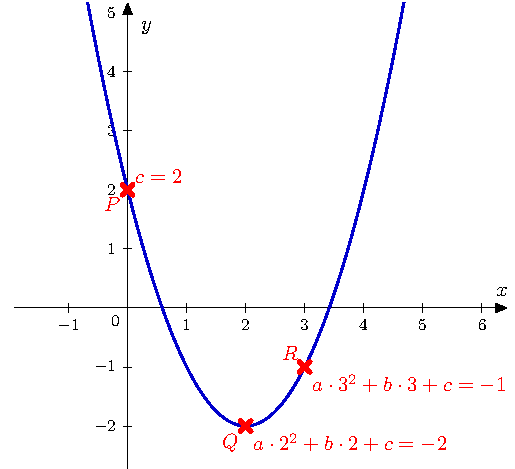
\includegraphics[width=\textwidth]{./parabelfit.pdf}
 % parabelfit.pdf: 0x0 pixel, 300dpi, 0.00x0.00 cm, bb=
 \caption{Parabel durch drei Punkte}
 \label{fig:parabelfit}
\end{figure}
 Gegeben seien die drei Punkte \(P(0|2)\), \(Q(2|-2)\) und \(R(3|-1)\). Gesucht ist die quadratische Funktion, deren Graph durch diese drei Punkte verläuft.
 
 In den Ansatz \(f(x)=ax^2+bx+c=y\) werden die Koordinaten eingesetzt:
 \begin{align*}
  \text{I} && a\cdot 0^2 + b\cdot 0 +c &= 2 \\
  \text{II} && a\cdot 2^2 + b \cdot 2 + c &= -2 \\
  \text{III} && a\cdot 3^2 + b \cdot 3 + c &= -1 
 \end{align*}
 Aus Gleichung~I folgt sofort \(c=2\). Einsetzen in die anderen beiden Gleichungen liefert:
 \begin{align*}
  \text{II'} && 4a + 2b &= -4 \\
  \text{III'} && 9a + 3b &= -3
 \end{align*}
 Auflösen von II' nach \(b\):
 \begin{align*}
  2b &= -4-4a \\
  b &= -2-2a
 \end{align*}
 Einsetzen von \(b\) in III':
 \begin{align*}
  9a+3(-2-2a) &= -3\\
  9a-6-6a &= -3 \\
  3a &= 3 \\
  a&=1\\
  \intertext{Rückeinsetzen:}
  b &= -4
 \end{align*}

 Die gesuchte Funktionsgleichung ist also:
 \begin{equation*}
  f(x) = x^2-4x+2
 \end{equation*} 

\end{bsp}




\chapter{Geometrie der 9.~Jahrgangsstufe}
\epigraph{Wo Materie ist, dort ist auch Geometrie.}{\textit{De fundamentis astrologiae certioribus}\\\textsc{Johannes Kepler}}

\section{Satzgruppe des Pythagoras}

\textsc{Pythagoras von Samos} wurde um 570~v.Chr. geboren. Nachdem er Ägypten und Babylon bereist hatte, ließ er sich um 530~v.Chr. im Süden des heutigen Italien nieder und gründete dort einen Orden. Ziel des Ordens der \emph{Pythagoreer} war vor allem eine harmonische Lebensführung. Die Pythagoreer hatten starken politischen Einfluss und waren wirtschaftlich erfolgreich. Um 510~v.Chr. wurde Pythagoras aus Kroton vertrieben. Er ging mit seinen Anhängern nach Metapont, wo er auch starb. Er hinterließ seine Frau und seine Tochter \textsc{Myia}, die selbst zu einer bedeutenden Philosophin ihrer Zeit werden sollte.

Pythagoras unterrichtete seine Anhänger in Philosophie und Mathematik. Viele seiner Kenntnisse brachte er aber von seinen Reisen aus Babylon und Ägypten mit, sodass heute nicht mehr geklärt werden kann, was wirklich von ihm selbst entdeckt worden war. Der \emph{Satz des Pythagoras} war als Rechenvorschrift vermutlich schon den Babyloniern vor 1650~v.Chr. bekannt.\footnote{Die Keilschrifttafel \emph{Plimpton~322} enthält eine Tabelle pythatoreischer Tripel.} 

Die Sätze der \emph{Satzgruppe des Pythagoras} erlauben Berechnungen der Seitenlängen und der Höhe von rechtwinkligen Dreiecken. Sie sind nur auf rechtwinklige Dreiecke anwendbar.

Die längste Seite in einem rechtwinkligen Dreieck wird als \emph{Hypotenuse}\footnote{Der Begriff \emph{Hypotenuse} stammt von den altgriechischen Begriffen \emph{hypo} für "`unten"' und \emph{teinein} für "`spannen"' oder "`sich erstrecken"'.} bezeichnet. Die beiden kurzen Seiten heißen \emph{Katheten}. Der Mittelpunkt des Umkreises eines rechtwinkligen Dreiecks ist der Mittelpunkt der Hypotenuse. Diesen Umkreis nennt man den \emph{Thaleskreis}.

\begin{figure}\begin{center}
               \begin{tikzpicture}[x=1cm,y=1cm]
\draw (0,0)  coordinate (A)  -- node[below,sloped] { Hypotenuse \(c\)} (5,0) coordinate (B) -- node[above,sloped] {Kathete \(a\)} +(143.1:4) coordinate (C) -- node[above,sloped] {Kathete \(b\)} (A);
\draw (A) node[anchor=north east] (An){\(A\)};
\draw (B) node [anchor=north west] (Bn) {\(B\)};
\draw (C) node [anchor=south] (Cn) {\(C\)};
% \draw[dashed] (2.5,0) circle (2.5cm);
\path[draw=blue, dashed,
  postaction={decorate ,decoration={text along path,
    text={\ Thaleskreis\ }, text align=center,
    text effects/.cd,  
    every character/.style={fill=white, yshift=-0.5ex}}}]
  (2.5, 2.5) arc [start angle=-270, end angle=90, radius=2.5];

\clip (A)--(B)--(C);
\draw (C) circle (0.5cm);
\fill[black] (C) ++(-80:0.25) circle (1pt);
\draw (A) circle (1cm);
\draw (B) circle (1.5cm);
\draw (A) ++(30:0.6) node{\(\alpha\)};
\draw (B) ++(165:1) node{\(\beta\)};


\end{tikzpicture}\end{center}
\caption{Benennungen im rechtwinkligen Dreieck}
\end{figure}

\subsection{Kathetensatz}

\begin{ssatz}[Kathetensatz]
 Der Flächeninhalt des Quadrats über einer Kathete entspricht dem Flächeninhalt des Rechtecks über der Hypotenuse, dessen zweite Seitenlänge der zugehörige Hypotenusenabschnitt bildet.
 
 \begin{blockwhitebox}
 \begin{equation*}  a^2 = p\cdot c \qquad b^2 = q\cdot c
 \end{equation*}
 \end{blockwhitebox}
 
 \begin{figure}\begin{center}
               \begin{tikzpicture}[x=1cm,y=1cm]
\tkzDefPoint(0,0){A}
\tkzLabelPoint[left](A){$A$}
\tkzDefPoint(5,0){B}
\tkzLabelPoint[right](B){$B$}
\tkzDrawTriangle[two angles=30 and 60](A,B) \tkzGetPoint{C}
\tkzLabelPoint[above](C){$C$}
\tkzMarkRightAngle(A,C,B)
\tkzLabelSegment[below,sloped](A,B){$c$}
\tkzLabelSegment[below,sloped,red](B,C){$a$}
\tkzLabelSegment[above,sloped](A,C){$b$}

\tkzDrawAltitude(A,B)(C) \tkzGetPoint{H}
\tkzLabelPoint[above left](H){$H$}
\tkzLabelSegment[left](H,C){$h$}
\tkzMarkRightAngle(B,H,C)

\tkzDrawSquare[red](C,B) \tkzGetPoints{D}{E}
\tkzLabelSegment[above,red,sloped](E,C){$a$}
\tkzFillPolygon[red,opacity=0.2](C,B,D,E)
% \tkzDefMidPoint(C,D) \tkzGetPoint{M}
% \tkzDrawPoint(M)
% \tkzLabelPoint[](M){$a^2$}
\tkzLabelSegment[anchor=center,red](C,D){$a^2$}

\tkzDefSquare(B,H) \tkzGetPoints{H1}{H2}
\tkzDrawArc[color=gray,towards,delta=10](B,H)(H2)

\tkzDefLine[orthogonal=through A](B,H) \tkzGetPoint{H3}
% \tkzInterLL(H1,H2)(A,H3) \tkzGetPoint{H4}
\tkzDrawPolygon[red](A,H3,H2,B)
\tkzFillPolygon[red,opacity=0.2](A,H3,H2,B)

\tkzLabelSegment[right,red](H2,B){$p$}
\tkzLabelSegment[below,red](H2,H3){$c$}

\begin{scope}[yshift=4cm, scale=0.4]
\tkzDefPoint(0,0){A2}
\tkzLabelPoint[left](A2){$A$}
\tkzDefPoint(5,0){B2}
\tkzLabelPoint[right](B2){$B$}
\tkzDrawTriangle[two angles=30 and 60](A2,B2) \tkzGetPoint{C2}
\tkzLabelPoint[above](C2){$C$}
\tkzMarkRightAngle(A2,C2,B2)
\tkzLabelSegment[below,sloped](A2,B2){$c$}
\tkzLabelSegment[above,sloped](B2,C2){$a$}
\tkzLabelSegment[below,sloped,green!50!black](A2,C2){$b$}

\tkzDrawAltitude(A2,B2)(C2) \tkzGetPoint{I}
% \tkzLabelPoint[above left](I){$H$}
% \tkzLabelSegment[left](I,C2){$h$}
\tkzMarkRightAngle(B2,I,C2)

\tkzDrawSquare[green!50!black](A2,C2) \tkzGetPoints{D2}{E2}
\tkzLabelSegment[above,green!50!black,sloped](D2,C2){$b$}
\tkzFillPolygon[green,opacity=0.2](A2,C2,D2,E2)
\tkzLabelSegment[anchor=center,green!50!black](A2,D2){$b^2$}

\tkzDefSquare(I,A2) \tkzGetPoints{I1}{I2}
\tkzDrawArc[color=gray,towards,delta=10](A2,I1)(I)

\tkzDefLine[orthogonal=through B2](I,A2) \tkzGetPoint{I3}
% \tkzInterLL(H1,H2)(A,H3) \tkzGetPoint{H4}
\tkzDrawPolygon[green!50!black](A2,I1,I3,B2)
\tkzFillPolygon[green,opacity=0.2](A2,I1,I3,B2)

 \tkzLabelSegment[left,green!50!black](I1,A2){$q$}
 \tkzLabelSegment[below,green!50!black](I1,I3){$c$}
\end{scope}
\end{tikzpicture}

\end{center}
\caption{Veranschaulichung des Kathetensatzes}
\end{figure}
\end{ssatz}

\begin{bew}
 Der Kathetensatz ergibt sich aus der Ähnlichkeit des Dreiecks \(\triangle ABC\) zum Dreieck \(\triangle CBH\). Diese Dreiecke sind ähnlich, da sie zwei Winkel gemeinsam haben: Den rechten Winkel bei \(C\) bzw. \(H\) und den Winkel \(\beta\).
 
 In diesen ähnlichen Dreiecken sind die Verhältnisse einander entsprechender Streckenlängen gleich. Also gilt:
 \begin{align*}
  \frac{p}{a} &= \frac{a}{c} && |\cdot a \cdot c \\
  pc &= a^2
 \end{align*}
 Einfaches Umformen der Gleichung der Seitenverhältnisse liefert also direkt den Kathetensatz.
\end{bew}

Der Beweis für den Kathetensatz für die Kathete \(b\) verläuft analog.

Mit Hilfe des Kathetensatzes lässt sich zu jedem Rechteck ein flächengleiches Quadrat konstruieren.

\begin{beme}[Flächengleiches Quadrat]
 Die Konstruktion eines flächengleichen Quadrats aus einem Rechteck mit gegebenen Seitenlägen \(c\) und \(p\) kann über die Anwendung des Kathetensatzes erfolgen. Es sei \(c=[AB]\). Folgende Konstruktionsschritte sind erforderlich:
 \begin{enumerate}
  \item Trage \(p\) an \(c\) ab. Das ergibt Punkt \(H\).
  \item Errichte einen Halbkreis \(k\) über \(c\).
  \item Errichte das Lot \(h\) zu \(c\) durch \(H\).
  \item Der Schnittpunkt von \(h\) mit \(k\) ergibt den Punkt \(C\). Das Quadrat über \([CB]\) hat den gleichen Flächeninhalt.
 \end{enumerate}
\end{beme}


\subsection{Satz des Pythagoras}

\begin{ssatz}[Satz des Pythagoras]
 Der Flächeninhalt des Quadrats über der Hypotenuse entspricht der Summe der Flächeninhalte der Quadrate über den Katheten.
  \begin{blockwhitebox}
 \begin{equation*}  a^2 + b^2 = c^2
 \end{equation*}
 \end{blockwhitebox}
   \begin{figure}\begin{center}
               \begin{tikzpicture}[x=1cm,y=1cm,scale=0.8]
\tkzDefPoint(0,0){A}
\tkzLabelPoint[left](A){$A$}
\tkzDefPoint(5,0){B}
\tkzLabelPoint[below right](B){$B$}
\tkzDrawTriangle[two angles=30 and 60](A,B) \tkzGetPoint{C}
\tkzLabelPoint[above](C){$C$}
\tkzMarkRightAngle(A,C,B)
\tkzLabelSegment[below,sloped](A,B){$c$}
\tkzLabelSegment[above,sloped](B,C){$a$}
\tkzLabelSegment[above,sloped](A,C){$b$}

\tkzDrawAltitude(A,B)(C) \tkzGetPoint{H}
% \tkzLabelPoint[above left](H){$H_c$}
\tkzLabelSegment[left](H,C){$h$}
\tkzMarkRightAngle(B,H,C)

\tkzDrawSquare[red](C,B) \tkzGetPoints{D}{E}
\tkzLabelSegment[above,red,sloped](E,C){$a$}
\tkzFillPolygon[red,opacity=0.2](C,B,D,E)
\tkzLabelSegment[anchor=center,red](C,D){$a^2$}

\tkzDrawSquare[green!50!black](A,C) \tkzGetPoints{D2}{E2}
\tkzLabelSegment[above,green!50!black,sloped](D2,C){$b$}
\tkzFillPolygon[green,opacity=0.2](A,C,D2,E2)
\tkzLabelSegment[anchor=center,green!50!black](A,D2){$b^2$}

\tkzDrawSquare[blue](B,A) \tkzGetPoints{F}{G}
\tkzLabelSegment[left,blue](A,F){$c$}
\tkzFillPolygon[blue,opacity=0.2](A,F,G,B)
\tkzLabelSegment[anchor=center,blue](A,G){$c^2$}

\end{tikzpicture}\end{center}
\caption{Veranschaulichung des Satz des Pythagoras}
\end{figure}
\end{ssatz}

Für den Satz des Pythagoras sind heute über 400 verschiedene Beweise bekannt. Eine kleine Auswahl wird hier präsentiert.

\begin{bew}[Arithmetischer Beweis]

Über der Hypotenuse des rechtwinkligen Dreiecks \(\triangle ABC\) wird das Quadrat errichtet. An die anderen drei Seiten dieses Quadrats wird wieder das Ausgangsdreieck nach innen angefügt.
\begin{figure}\begin{center}
               \begin{tikzpicture}[x=1cm,y=1cm,scale=0.8]
\tkzDefPoint(0,0){A}
\tkzLabelPoint[below left](A){$A$}
\tkzDefPoint(5,0){B}
\tkzLabelPoint[below right](B){$B$}
\tkzDrawTriangle[two angles=30 and 60](A,B) \tkzGetPoint{C}
\tkzLabelPoint[above right](C){$C$}
\tkzMarkRightAngle(A,C,B)
\tkzLabelSegment[below,sloped](A,B){$c$}
\tkzLabelSegment[below,sloped](B,C){$a$}
\tkzLabelSegment[below,sloped](A,C){$b$}

\tkzDrawSquare[](A,B)\tkzGetPoints{A2}{B2}
\tkzLabelPoint[above right](A2){$A'$}
\tkzLabelPoint[above left](B2){$B'$}
\tkzDrawTriangle[two angles=30 and 60](B,A2) \tkzGetPoint{C2}
\tkzLabelPoint[above left](C2){$D$}
\tkzMarkRightAngle(B,C2,A2)
\tkzDrawTriangle[two angles=30 and 60](A2,B2) \tkzGetPoint{C3}
\tkzLabelPoint[below left](C3){$E$}
\tkzMarkRightAngle(A2,C3,B2)
\tkzDrawTriangle[two angles=30 and 60](B2,A) \tkzGetPoint{C4}
\tkzLabelPoint[below right](C4){$F$}
\tkzMarkRightAngle(B2,C4,A)
\tkzFillPolygon[red,opacity=0.2](C,C2,C3,C4)

\tkzDefMidPoint(C,C3)\tkzGetPoint{M}
\tkzLabelPoint[anchor=center,red](M){$(b-a)^2$}

 \end{tikzpicture}\end{center}
\caption{Figur zum Arithmetischen Beweis des Satz des Pythagoras}
\end{figure}
Daraus ergibt sich das neue Quadrat \(\square CDEF\) mit dem Flächeninhalt:
\begin{align*}
 A_{\square CDEF} &= (b-a)^2 = b^2 -2ab +a^2
\end{align*}
Den Flächeninhalt von \(\square CDEF\) kann man aber auch auf eine zweite Weise bestimmen. Diesen Flächeninhalt erhält man, wenn man vom Hypotenusenquadrat \(\square ABA'B'\) viermal die Fläche des Ausgangsdreicks \(\triangle ABC\) subtrahiert.
\begin{align*}
 A_{\square CDEF} &= A_{\square ABA'B'} - 4\cdot A_{\triangle ABC} \\
 &= c^2 - 4\cdot \frac{1}{2}ab \\
 \intertext{Einsetzen des ersten Terms:}
 (b-a)^2 &= c^2 - 2ab \\
 b^2 -2ab + a^2 &= c^2 - 2ab && | +2ab \\
 b^2 + a^2 &= c^2
\end{align*}

\end{bew}

\begin{bew}[Chinesischer Ergänzungsbeweis]
  Die\-se Vi\-su\-a\-li\-sie\-rung -- kein echter Beweis im logischen Sinn -- findet man im Kommentar zum ersten Buch von Euklids \emph{Elementen} von \textsc{Proklos}, in hinduistischen Schriften und im chinesischen \emph{Zhoubi suanjing} (ca.~100~v.Chr.). Dieser Nachweis ergänzt zum Ausgangsdreieck kongruente Dreiecke außen an das Hypotenusenquadrat. Das sich ergebende Quadrat \(\square CDEF\) lässt sich dann durch eine Umordnung der vier kongruenten Dreiecke innerhalb seiner Fläche auch in zwei Rechtecke mit den Seitenlängen \(a\) und \(b\), sowie in zwei Quadrate mit den Flächeninhalten \(a^2\) und \(b^2\) zerlegen.\footnote{Auch bekannt als \emph{Altindischer Ergänzungsbeweis}}
 \begin{figure}\begin{center}
               \begin{tikzpicture}[x=1cm,y=1cm,scale=0.8]
\begin{scope}[xshift=-2.5cm, scale=0.4]                              
\tkzDefPoint(0,0){A}
% \tkzLabelPoint[below left](A){$A$}
\tkzDefPoint(5,0){B}
% \tkzLabelPoint[below right](B){$B$}
\tkzDrawTriangle[two angles=30 and 60](A,B) \tkzGetPoint{C}
\tkzLabelPoint[above](C){$C$}
\tkzMarkRightAngle(A,C,B)
% \tkzLabelSegment[above,sloped](A,B){$c$}
\tkzLabelSegment[above,sloped](B,C){$a$}
\tkzLabelSegment[above,sloped](A,C){$b$}

\tkzDrawSquare[](B,A)\tkzGetPoints{A2}{B2}
% \tkzLabelPoint[above right](A2){$A'$}
% \tkzLabelPoint[above left](B2){$B'$}
\tkzDrawTriangle[two angles=30 and 60](A2,A) \tkzGetPoint{C2}
\tkzLabelPoint[left](C2){$D$}
\tkzMarkRightAngle(A2,C2,A)
\tkzDrawTriangle[two angles=30 and 60](B2,A2) \tkzGetPoint{C3}
\tkzLabelPoint[below](C3){$E$}
\tkzMarkRightAngle(B2,C3,A2)
\tkzDrawTriangle[two angles=30 and 60](B,B2) \tkzGetPoint{C4}
\tkzLabelPoint[right](C4){$F$}
\tkzMarkRightAngle(B,C4,B2)
\tkzFillPolygon[blue,opacity=0.2](A,A2,B2,B)

\tkzDefMidPoint(A,B2)\tkzGetPoint{M}
\tkzLabelPoint[anchor=center,blue](M){$c^2$}
\end{scope}
\begin{scope}[xshift=2.5cm, scale=0.4]                              
\tkzDefPoint(0,0){A}
% \tkzLabelPoint[below left](A){$A$}
\tkzDefPoint(5,0){B}
% \tkzLabelPoint[below right](B){$B$}
\tkzDrawTriangle[two angles=30 and 60](A,B) \tkzGetPoint{C}
\tkzLabelPoint[above](C){$C$}
\tkzMarkRightAngle(A,C,B)
% \tkzLabelSegment[below,sloped](A,B){$c$}
\tkzLabelSegment[above,sloped](B,C){$a$}
\tkzLabelSegment[above,sloped](A,C){$b$}
\tkzDefTriangle[two angles=30 and 60](B,A) \tkzGetPoint{D}
\tkzMarkRightAngle(B,D,A)
\tkzDrawSquare[](D,A)\tkzGetPoints{E}{F}
\tkzLabelPoint[left](E){$D$}
\tkzDrawSquare[](B,D)\tkzGetPoints{G}{H}
\tkzDrawTriangle[two angles=60 and 30](G,F) \tkzGetPoint{I}
\tkzMarkRightAngle(F,D,G)
\tkzMarkRightAngle(G,I,F)
\tkzLabelPoint[below](I){$E$}
\tkzLabelPoint[right](H){$F$}
\tkzFillPolygon[red,opacity=0.2](A,E,F,D)
\tkzFillPolygon[green,opacity=0.2](B,D,G,H)
\tkzDefMidPoint(A,F)\tkzGetPoint{M}
\tkzLabelPoint[anchor=center,red](M){$a^2$}
\tkzDefMidPoint(B,G)\tkzGetPoint{N}
\tkzLabelPoint[anchor=center,green!50!black](N){$b^2$}
\end{scope}
 \end{tikzpicture}\end{center}
 \caption{Figur zum Chinesischen Ergänzungsbeweis des Satz des Pythagoras}
\end{figure}
Stellt man den Term für die Fläche von \(\square CDEF\) auf, erhält man:
 \begin{align*}
  A_{\square CDEF} &= c^2 + 4 \cdot \frac{1}{2}ab \\
  \intertext{aber auch:}
  A_{\square CDEF} &= a^2 + b^2 + 2ab \\
  \intertext{Gleichsetzen liefert:}
  c^2 + 2ab &= a^2 + b^2 + 2ab \\
  c^2 &= a^2 + b^2
 \end{align*}
\end{bew}


\begin{bew}[Beweis nach \textsc{Euklid}]

Der nächste Beweis ist im ersten Buch der Elemente des \textsc{Euklid} zu finden. Der Beweis fußt auf einer Abfolge von drei flächenerhaltenden Transformationen.\footnote{flächenerhaltende Transformationen sind: Verschiebung, Drehung, Spiegelung und Scherung.}

 \begin{figure}\begin{center}
               \begin{tikzpicture}[x=1cm,y=1cm,scale=0.8]
               \small
\begin{scope}[xshift=-2.5cm, yshift=2.5cm, scale=0.4]                              
\tkzDefPoint(0,0){A}
\tkzLabelPoint[below left](A){$A$}
\tkzDefPoint(5,0){B}
\tkzLabelPoint[below right](B){$B$}
\tkzDrawTriangle[two angles=30 and 60](A,B) \tkzGetPoint{C}
\tkzLabelPoint[above](C){$C$}
\tkzMarkRightAngle(A,C,B)
% \tkzLabelSegment[below,sloped](A,B){$c$}
% \tkzLabelSegment[below,sloped](B,C){$a$}
% \tkzLabelSegment[below,sloped](A,C){$b$}

\tkzDrawSquare[](A,C)\tkzGetPoints{D}{E}
\tkzLabelPoint[above ](D){$D$}
\tkzLabelPoint[above left](E){$E$}
\tkzDefMidPoint(A,D)\tkzGetPoint{M}
\tkzLabelPoint[anchor=center,green!50!black](M){$b^2$}
\tkzFillPolygon[green,opacity=0.2](A,C,D,E)

\tkzDrawSquare[](C,B)\tkzGetPoints{F}{G}
\tkzLabelPoint[above ](G){$G$}
\tkzLabelPoint[above right](F){$F$}
\tkzDefMidPoint(B,G)\tkzGetPoint{N}
\tkzLabelPoint[anchor=center,red](N){$a^2$}
\tkzFillPolygon[red,opacity=0.2](C,B,F,G)
\tkzInterLL(E,D)(G,F) \tkzGetPoint{P}
\tkzDrawVector[gray](D,P)
\tkzDrawVector[gray](G,P)
\end{scope}
\begin{scope}[xshift=2.5cm,yshift=2.5cm, scale=0.4]                              
\tkzDefPoint(0,0){A2}
% \tkzLabelPoint[below left](A){$A$}
\tkzDefPoint(5,0){B2}
% \tkzLabelPoint[below right](B){$B$}
\tkzDrawTriangle[two angles=30 and 60](A2,B2) \tkzGetPoint{C2}
% \tkzLabelPoint[below](C2){$C$}
\tkzMarkRightAngle(A2,C2,B2)
\tkzDrawAltitude[dashed](A2,B2)(C2) \tkzGetPoint{H2}
\tkzDrawSquare[](A2,C2)\tkzGetPoints{D2}{E2}
\tkzDrawSquare[](C2,B2)\tkzGetPoints{F2}{G2}
\tkzInterLL(E2,D2)(G2,F2) \tkzGetPoint{P2}
\tkzLabelPoint[above](P2){$P$}
\tkzDefLine[orthogonal=through A2](A2,B2) \tkzGetPoint{Y2}
\tkzInterLL(E2,D2)(A2,Y2) \tkzGetPoint{R2}
\tkzFillPolygon[green,opacity=0.2](A2,C2,P2,R2)

\tkzDefLine[orthogonal=through B2](A2,B2) \tkzGetPoint{Z2}
\tkzInterLL(F2,G2)(B2,Z2) \tkzGetPoint{S2}
\tkzFillPolygon[red,opacity=0.2](C2,B2,Z2,P2)

\tkzDrawSegment[dashed](C2,P2)
\tkzDrawSegment[dashed](D2,P2)
\tkzDrawSegment[dashed](G2,P2)
\tkzDrawSegment[dotted](A2,Y2)
\tkzDrawSegment[dotted](B2,Z2)
\end{scope}
\begin{scope}[xshift=+2.5cm,yshift=-2cm, scale=0.4]                              
\tkzDefPoint(0,0){A3}
% \tkzLabelPoint[below left](A){$A$}
\tkzDefPoint(5,0){B3}
% \tkzLabelPoint[below right](B){$B$}
\tkzDrawTriangle[two angles=30 and 60](A3,B3) \tkzGetPoint{C3}
% \tkzLabelPoint[below](C2){$C$}
\tkzMarkRightAngle(A3,C3,B3)
\tkzDrawAltitude[dashed](A3,B3)(C3) \tkzGetPoint{H3}
\tkzLabelPoint[below](H3){$H$}
\tkzDrawSquare[](A3,C3)\tkzGetPoints{D3}{E3}
\tkzDrawSquare[](C3,B3)\tkzGetPoints{F3}{G3}
\tkzInterLL(E3,D3)(G3,F3) \tkzGetPoint{P3}
\tkzDefLine[orthogonal=through A3](A3,B3) \tkzGetPoint{Y3}
\tkzInterLL(E3,D3)(A3,Y3) \tkzGetPoint{R3}

\tkzDefLine[orthogonal=through B3](A3,B3) \tkzGetPoint{Z3}
\tkzInterLL(F3,G3)(B3,Z3) \tkzGetPoint{S3}
\tkzInterLL(C3,H3)(Y3,Z3) \tkzGetPoint{T3}
\tkzFillPolygon[green,opacity=0.2](A3,H3,T3,Y3)
\tkzFillPolygon[red,opacity=0.2](H3,B3,Z3,T3)

\tkzDrawSegment[dashed](C3,P3)
\tkzDrawSegment[dashed](D3,P3)
\tkzDrawSegment[dashed](G3,P3)
\tkzDrawSquare[dotted](A3,B3)
\end{scope}
\begin{scope}[xshift=-2.5cm,yshift=-2cm, scale=0.4]                              
\tkzDefPoint(0,0){A4}
% \tkzLabelPoint[below left](A){$A$}
\tkzDefPoint(5,0){B4}
% \tkzLabelPoint[below right](B){$B$}
\tkzDrawTriangle[two angles=30 and 60](A4,B4) \tkzGetPoint{C4}
% \tkzLabelPoint[below](C2){$C$}
\tkzMarkRightAngle(A4,C4,B4)
\tkzDrawAltitude[dashed](A4,B4)(C4) \tkzGetPoint{H4}
\tkzDrawSquare[](A4,C4)\tkzGetPoints{D4}{E4}
\tkzDrawSquare[](C4,B4)\tkzGetPoints{F4}{G4}
\tkzInterLL(E4,D4)(G4,F4) \tkzGetPoint{P4}
\tkzDefLine[orthogonal=through A4](A4,B4) \tkzGetPoint{Y4}
\tkzInterLL(E4,D4)(A4,Y4) \tkzGetPoint{R4}

\tkzDefLine[orthogonal=through B4](A4,B4) \tkzGetPoint{Z4}
\tkzInterLL(F4,G4)(B4,Z4) \tkzGetPoint{S4}
\tkzInterLL(C4,H4)(Y4,Z4) \tkzGetPoint{T4}
\tkzDrawSquare[blue](B4,A4)\tkzGetPoints{I4}{J4}
\tkzInterLL(C4,H4)(I4,J4) \tkzGetPoint{Q4}

\tkzFillPolygon[green,opacity=0.2](A4,I4,Q4,H4)
\tkzFillPolygon[red,opacity=0.2](H4,Q4,J4,B4)

\tkzDrawSegment[dashed](C4,P4)
\tkzDrawSegment[dashed](D4,P4)
\tkzDrawSegment[dashed](G4,P4)
\tkzDrawSquare[dotted](A4,B4)
\end{scope}
\tkzDrawVector[gray](P,P2)
\tkzLabelSegment[sloped,above,gray](P,P2){Scherung}
\tkzDrawVector[gray](C2,T3)
\tkzLabelSegment[right,gray](C2,T3){Scherung}
\tkzDrawVector[gray](T3,H4)
\tkzLabelSegment[sloped,above,fill=white,opacity=0.5](T3,H4){Verschiebung}

\end{tikzpicture}\end{center}
 \caption{Beweis nach \textsc{Euklid}}
\end{figure}

Ausgangspunkt ist das rechtwinklige Dreieck über dessen Katheten die Quadrate errichtet werden. Im ersten Schritt werden die Quadrate einer Scherung entlang von Parallelen zu den Katheten unterzogen, sodass die Punkte \(D\) und \(G\) auf dem Punkt \(P\) zu liegen kommen. \(P\) befindet sich in der Verlängerung der Höhe von Dreieck \(\triangle ABC\). So erhält man zwei Parallelogramme, die eine Seite gemeinsam haben. Die Parallelogramme haben die Flächeninhalte \(a^2\) und \(b^2\).

Der zweite Schritt besteht darin, dass die Parallelogramme ein zweites Mal einer Scherung unterzogen werden. Dabei kommt der Punkt \(C\) auf dem Höhenfußpunkt \(H\) zu liegen. Man erhält zwei Rechtecke, die gemeinsam ein Quadrat ergeben, dessen Seitenlänge der Hypotenuse \(c\) entspricht.

Um zuletzt noch zu zeigen, dass das Quadrat, das durch die beiden Scherungen entstanden ist, das Hypotenusenquadrat ist, kann man es noch nach unten verschieben.

Da weder Scherung noch Verschiebung einen Flächeninhalt ändern, folgt daraus, dass \(a^2+b^2 = c^2\).

\end{bew}

\begin{satz}[Umkehrung des Satz des Pythagoras]
 Ergibt die Summe der Quadrate zweier Seitenlängen im Quadrat das Quadrat der dritten Seitenlänge, so ist das Dreieck ein rechtwinkliges. Kurz:
 \begin{align*}
  a^2+b^2&=c^2&&\Rightarrow & \triangle ABC & \quad\text{ ist rechtwinklig.} 
 \end{align*}
\end{satz}

\begin{defi}[Pythagoreisches Tripel]
 Unter einem \emph{Pythagoreischen Tripel} versteht man eine Menge von drei ganzen Zahlen, die den Satz des Pythagoras erfüllen. Das bekannteste solche Tripel ist \((3,4,5)\), denn:
 \begin{equation*}
  3^2+4^2 = 9 +16 =25 =5^2
 \end{equation*}
 Andere Pythagoreische Tripel sind: \((5;12;13)\), \((8;15;17)\) oder \((20;21;29)\).
\end{defi}


\begin{beme}
 Auf der Umkehrung des Satz des Pythagoras beruht auch die oft von Handwerkern benutzte 3-4-5-Regel: Verhalten sich die in einem Dreieck die Seitenlägen wie 3 zu 4 zu 5, dann handelt es sich um ein rechtwinkliges.
\end{beme}


\subsection{Höhensatz}

\begin{ssatz}[Höhensatz]
   Der Flächeninhalt des Quadrats über der Höhe eines rechtwinkligen Dreiecks entspricht dem Flächeninhalt des Rechtecks der Hypotenusenabschnitte.
    \begin{blockwhitebox}
 \begin{equation*} h^2 = p\cdot q
 \end{equation*}
 \end{blockwhitebox}
 \begin{figure}\begin{center}
               \begin{tikzpicture}[x=1cm,y=1cm]\tkzInit[xmin=0, ymin=-1.5,xmax=6.5, ymax=2.5] \tkzClip[space=.5]
\tkzDefPoint(0,0){A}
\tkzLabelPoint[left](A){$A$}
\tkzDefPoint(5,0){B}
\tkzLabelPoint[below right](B){$B$}
\tkzDrawTriangle[two angles=30 and 60](A,B) \tkzGetPoint{C}
\tkzLabelPoint[above](C){$C$}
\tkzMarkRightAngle(A,C,B)
\tkzLabelSegment[below,sloped](A,B){$c$}
\tkzLabelSegment[above,sloped](B,C){$a$}
\tkzLabelSegment[above,sloped](A,C){$b$}

\tkzDrawAltitude(A,B)(C) \tkzGetPoint{H}
% \tkzLabelPoint[above left](H){$H_c$}
\tkzLabelSegment[left,red](H,C){$h$}
\tkzMarkRightAngle(B,H,C)

\tkzDrawSquare[red](C,H) \tkzGetPoints{D}{E}
\tkzLabelSegment[above,red](E,C){$h$}
\tkzFillPolygon[red,opacity=0.2](C,H,D,E)


\tkzDefSquare(B,H) \tkzGetPoints{H1}{H2}
\tkzDrawArc[color=gray,towards,delta=10](H,H1)(B)

\tkzDefLine[orthogonal=through A](A,B) \tkzGetPoint{H3}
\tkzInterLL(H1,H2)(A,H3) \tkzGetPoint{H4}
\tkzDrawPolygon[red](H,H1,H4,A)
\tkzFillPolygon[red,opacity=0.2](H,H1,H4,A)

\tkzLabelSegment[below,red](H4,H1){$q$}
\tkzLabelSegment[right,red](H,H1){$p$}

\end{tikzpicture}\end{center}
\caption{Veranschaulichung des Höhensatzes}
\end{figure}
\end{ssatz}

\begin{bew}[Ergänzungsbeweis]
 Der Höhensatz lässt sich dadurch zeigen, dass man die Figur zu einem Rechteck ergänzt. (s. Abb.~\ref{abb:bewHSatz}) Betrachte dann das Dreieck \(\triangle PQR\). Sein Flächeninhalt lässt sich auf zwei Arten berechnen. Einerseits entspricht der Flächeninhalt der Hälfte des Rechtecks mit den Seitenlängen \(q+h\) und \(p+h\). Andererseits setzt sich das Dreiecks aus dem Rechteck mit den Seitenlängen \(p\) und \(q\), sowie den Hälften der Rechtecke mit den Seitenlängen \(q\) und \(h\) bzw. \(p\) und \(h\) zusammen.
 \begin{figure}\begin{center}
               \begin{tikzpicture}[x=1cm,y=1cm]
\tkzInit[xmin=0, ymin=-3,xmax=5, ymax=2.5] \tkzClip[space=.5]
\tkzDefPoint(0,0){A}
\tkzLabelPoint[left](A){$A$}
\tkzDefPoint(5,0){B}
\tkzLabelPoint[below right](B){$B$}
\tkzDrawTriangle[two angles=50 and 40](A,B)\tkzGetPoint{C}
\tkzLabelPoint[above](C){$C$}
\tkzMarkRightAngle(A,C,B)
% \tkzLabelSegment[below,sloped](A,B){$c$}
% \tkzLabelSegment[above,sloped](B,C){$a$}
% \tkzLabelSegment[above,sloped](A,C){$b$}

\tkzDrawAltitude(A,B)(C) \tkzGetPoint{H}
% \tkzLabelPoint[above left](H){$H_c$}
% \tkzLabelSegment[left,red](H,C){$h$}
\tkzMarkRightAngle(B,H,C)

\tkzDrawSquare[red](C,H) \tkzGetPoints{D}{E}
\tkzLabelSegment[above,red](E,C){$h$}
\tkzLabelSegment[right,red](D,E){$h$}
\tkzFillPolygon[red,opacity=0.2](C,H,D,E)

\tkzDefSquare(B,H) \tkzGetPoints{H1}{H2}
\tkzDrawArc[color=gray,towards,delta=10](H,H1)(B)

\tkzDefLine[orthogonal=through A](A,B) \tkzGetPoint{H3}
\tkzInterLL(H1,H2)(A,H3) \tkzGetPoint{H4}
% \tkzLabelPoint(H4){$H_4$}
% \tkzLabelPoint(H1){$H_1$}
% \tkzLabelPoint(D){$D$}
% \tkzLabelPoint(E){$E$}
\tkzDrawPolygon[red](H,H1,H4,A)
\tkzFillPolygon[red,opacity=0.2](H,H1,H4,A)

\tkzLabelSegment[below,red](H4,H1){$q$}
\tkzLabelSegment[left,red](A,H4){$p$}

\tkzInterLL(H2,H1)(E,D) \tkzGetPoint{G}
% \tkzLabelPoint(G){$G$}
\tkzDrawPolygon[green](D,H,H1,G)
\tkzFillPolygon[green,opacity=0.2](D,H,H1,G)
\tkzInterLL(H4,A)(E,C) \tkzGetPoint{P}
\tkzDrawPolygon[blue](A,H,C,P)
\tkzFillPolygon[blue,opacity=0.2](A,H,C,P)
\tkzDrawSegment[dotted](P,G)

\tkzLabelSegment[below,green!50!black](H1,G){$h$}
\tkzLabelSegment[right,green!50!black](D,G){$p$}
\tkzLabelSegment[above,blue](P,C){$q$}
\tkzLabelSegment[left,blue](A,P){$h$}
\tkzLabelPoint[above left](P){$P$}
\tkzLabelPoint[below left](H4){$Q$}
\tkzLabelPoint[below right](G){$R$}
\end{tikzpicture}\end{center}
\caption{Beweisfigur zum Höhensatz}
\label{abb:bewHSatz}
\end{figure}
\begin{align*}
 A_{\triangle PQR} = \frac{1}{2} (p+h)(q+h) &= pq + \frac{1}{2}qh + \frac{1}{2}ph \\
                     \frac{1}{2} \left(pq +ph +qh + h^2\right) &= pq + \frac{1}{2}qh + \frac{1}{2}ph \\
                     \frac{1}{2} pq + \frac{1}{2} ph + \frac{1}{2} qh + \frac{1}{2} h^2 &= pq + \frac{1}{2}qh + \frac{1}{2}ph \\
                     \frac{1}{2} h^2 &= \frac{1}{2} pq \\
                     h^2 &= pq
\end{align*}

\end{bew}

\subsection{Dreiecksberechnungen}

\begin{folg}[Berechnung der Hypotenuse]
 Aus dem Satz des Pythagoras folgt: In einem rechtwinkligen Dreieck \(\triangle ABC\) gilt für die Länge der Hypotenuse \(c\):
 \begin{align*}
  c^2 &= a^2 + b^2 &&|\sqrt{\ldots}\\
  c &= \sqrt{a^2 + b^2}
 \end{align*}
 Die Längen der Katheten legen also die Länge der Hypotenuse fest.
\end{folg}

\begin{folg}[Berechnung der Höhe]
 Die Höhe eines rechtinkligen Dreiecks kann über verschiedene Wege bestimmt werden.
 
 Sind die Hypotenusenabschnitte gegeben, so lässt sich direkt der Höhensatz anwenden.
 \begin{align*}
  h^2 &= pq & &\Rightarrow & h &=\sqrt{pq}
 \end{align*}
 
 Ist eine Kathete und der zugehörige Hypotenusenabschnitt gegeben, so gilt nach dem Satz des Pythagoras für das Teildreieck \(\triangle ACH\) oder \(\triangle BHC\):
 \begin{align*}
  h^2 + p^2 &= a^2 & &\Rightarrow& h &=\sqrt{a^2-p^2} \\
  \intertext{analog:}
  h^2 + q^2 &= b^2 & &\Rightarrow& h &=\sqrt{b^2-q^2}
 \end{align*}
\end{folg}

\begin{folg}[Berechnung der Kathetenlänge]
 Die Länge einer der Katheten kann auch über mehrere Wege, abhängig von den gegebenen Größen erfolgen:
 
 Ist die Länge der Hypotenuse \(c\) und die Länge einer Kathete \(b\) bekannt, so kann der Satz des Pythagoras angewendet werden.
 \begin{align*}
  a^2 +b^2 &= c^2 & &\Rightarrow & a &=\sqrt{c^2-b^2}
 \end{align*}
 
 Ist ein Hypotenusenabschnitt, z.B. \(p\), und die Länge der Hypotenuse \(c\) bekannt, so kann die Länge der Katheten über den Kathetensatz berechnet werden.
 \begin{align*}
  a^2 &= pc &&\Rightarrow & a&=\sqrt{pc}\\
  b^2 &= qc = (c-p)c &&\Rightarrow & b&=\sqrt{(c-p)c}
 \end{align*}
 
 Ist die Höhe \(h\) und der passende Hyptenusenabschnitt, z.B. \(p\), bekannt, so kann die Länge der Katheten auch über den Satz des Pythagoras bestimmt werden.
 \begin{align*}
  a^2 &= h^2 + p^2 && \Rightarrow & a &= \sqrt{h^2+p^2}
 \end{align*}

\end{folg}

\begin{folg}[Gleichschenkliges Dreieck]
 An einem gleichschenkligen Dreieck ist keiner der Sätze aus der Satzgruppe des Pythagoras direkt anwendbar. Doch die Höhe auf die Basis des gleichschenkligen Dreiecks teil das Dreieck in zwei rechtwinklige Dreiecke. In diesen Teildreiecken sind Satz des Pythagoras, Katheten- und Höhensatz anwendbar.
 \begin{figure}
  \begin{center}
   \begin{tikzpicture}[x=1cm,y=1cm,scale=0.6]
 \tkzInit[xmin=-0.5, ymin=-0.5,xmax=3.5, ymax=5]
   \tkzClip[space=.3]
\tkzDefPoint(0,0){A} \tkzDefPoint(3,0){B}
\tkzDefTriangle[euclide](A,B)\tkzGetPoint{C}
\tkzDrawPolygon(A,B,C)
\tkzDrawPoints(A,B,C)
\tkzLabelPoint[left](A){$A$}
\tkzLabelPoint[right](B){$B$}
\tkzLabelPoint[above](C){$C$}
\tkzLabelSegment[below](A,B){$c$}
\tkzLabelSegment[above,sloped](A,C){$a$}
\tkzLabelSegment[above,sloped](B,C){$a$}
\tkzSetUpLine[color=red]
\tkzDrawBisector(A,C,B) \tkzGetPoint{H}
\tkzMarkRightAngle(B,H,C)
\tkzLabelPoint[red,above right](H){$H$}
\tkzLabelSegment[red,left,near end](C,H){$h$}
   \end{tikzpicture}
  \end{center}
  \caption{Gleichschenkliges Dreieck}
 \end{figure}
 So lässt sich die Höhe des gleichschenkligen Dreiecks aus den Seitenlängen berechnen. Betrachte das Dreieck \(\triangle HBC\). An diesem Dreieck gilt der Satz des Pythagoras:
 \begin{align*}
  \left(\frac{c}{2}\right)^2 + h^2 &= a^2 &&| -\left(\frac{c}{2}\right)^2 \\
  h^2 &= a^2-\frac{c^2}{4} && | \sqrt{\ldots} \\
  h &= \sqrt{a^2-\frac{c^2}{4}}
 \end{align*}
 
 Ist die Höhe des Dreiecks und die Basislänge \(c\) bekannt, so kann mit der gleichen Beziehung die Länge der beiden Schenkel berechnet werden:
 \begin{align*}
  a^2 &= \left(\frac{c}{2}\right)^2 + h^2 &&|\sqrt{\ldots}\\
  a &= \sqrt{\frac{c^2}{4}+h^2}
 \end{align*}
\end{folg}

\begin{folg}[Höhe im gleichseitigen Dreieck]
 Der Satz des Pythagoras verbindet im gleichseitigen Dreieck die Höhe des Dreiecks mit der Seitenlänge. Die Höhe teilt das Dreieck in zwei rechtwinklige Dreiecke.
 
  \begin{figure}
  \begin{center}
   \begin{tikzpicture}[x=1cm,y=1cm,scale=0.75]
 \tkzInit[xmin=-0.5, ymin=-0.2,xmax=3.5, ymax=3.5]
   \tkzClip[space=.3]
\tkzDefPoint(0,0){A} \tkzDefPoint(3,0){B}
\tkzDefTriangle[equilateral](A,B)\tkzGetPoint{C}
\tkzDrawPolygon(A,B,C)
\tkzDrawPoints(A,B,C)
\tkzLabelPoint[left](A){$A$}
\tkzLabelPoint[right](B){$B$}
\tkzLabelPoint[above](C){$C$}
\tkzLabelSegment[below](A,B){$a$}
\tkzLabelSegment[above,sloped](A,C){$a$}
\tkzLabelSegment[above,sloped](B,C){$a$}
\tkzSetUpLine[color=red]
\tkzDrawBisector(A,C,B) \tkzGetPoint{H}
\tkzMarkRightAngle(B,H,C)
\tkzLabelPoint[red,above right](H){$H$}
\tkzLabelSegment[red,left](C,H){$h$}
   \end{tikzpicture}
  \end{center}
  \caption{Gleichseitiges Dreieck}
 \end{figure}
 
 Betrachte das Dreieck \(\triangle HBC\). Der Satz des Pythagoras für dieses Dreieck lautet:
 \begin{align*}
  h^2 + \left(\frac{a}{2}\right)^2 &= a^2 && |- \left(\frac{a}{2}\right)^2 \\
  h^2 &= a^2 - \frac{a^2}{4} \\
  h^2 &= \frac{3}{4} a^2 &&| \sqrt{\ldots} \\
  h &= \sqrt{\frac{3}{4} a^2} = \frac{\sqrt{3}}{2}a
 \end{align*}
 
 Somit kann man auch den Flächeninhalt des gleichseitigen Dreiecks nur in Abhängigkeit der Seitenlänge ausdrücken.
 \begin{align*}
  A_{\triangle ABC} = \frac{1}{2} \cdot a\cdot h &= \frac{1}{2} \cdot a \cdot \frac{\sqrt{3}}{2}a \\
  &= \frac{\sqrt{3}}{4}a^2
 \end{align*}

\end{folg}


\subsection{Grundkonstruktionen}


\begin{regel}[Quadrat zu Rechteck]
Diese Grundkonstruktion erfüllt die Aufgabe ein Quadrat gegebener Fläche in ein \emph{flächengleiches} Rechteck umzuwandeln.
  \begin{figure}
  \begin{center}
   \begin{tikzpicture}[x=1cm,y=1cm,scale=0.5]
%  \tkzInit[xmin=-0.5, ymin=-0.2,xmax=3.5, ymax=3.5]
%    \tkzClip[space=.3]
\tkzDefPoint(0,0){A} \tkzDefPoint(3,0){B}
\tkzDrawSquare[red](A,B)\tkzGetPoints{C}{D}
\tkzDefPoint(3,4){E}
\tkzFillPolygon[red,opacity=0.2](A,B,C,D)
\tkzDrawPoints(A,B,C,D)
\tkzLabelPoint[left](A){$A$}
\tkzLabelPoint[right](B){$B$}
\tkzLabelPoint[below,right](C){$C$}
\tkzLabelPoint[left](D){$D$}
\tkzLabelSegment[below](A,B){$h$}
\tkzLabelSegment[above,sloped](A,D){$h$}
\tkzDrawCircle[dashed,color=gray](C,E)
\tkzInterLC(C,D)(C,E) \tkzGetPoints{F}{G}
\tkzDrawSegment(C,E)
\tkzLabelSegment[left](C,E){$p$}

\tkzDrawPoint(G)
\tkzDrawSegment(G,B)
\tkzDefLine[orthogonal=through B](B,G) \tkzGetPoint{H}
\tkzMarkRightAngle(H,B,G)
\tkzInterLL(D,C)(B,H) \tkzGetPoint{I}
\tkzDrawLine[add=.5 and 3.2](H,B)
\tkzDrawLine[add=.5 and 3.2](D,C)
\tkzDrawPoint(I)
\tkzDrawPoint(E)

\tkzDefLine[orthogonal=through I](D,C) \tkzGetPoint{J}
\tkzDefLine[orthogonal=through E](B,C) \tkzGetPoint{K}
\tkzInterLL(E,K)(I,J) \tkzGetPoint{L}
\tkzDrawPoint(L)
\tkzDrawPolygon[red](C,I,L,E)
\tkzFillPolygon[red,opacity=0.2](C,I,L,E)

\end{tikzpicture}
  \end{center}
  \caption{Flächenerhaltende Umformung eines Quadrats in ein Rechteck}
 \end{figure}

\end{regel}

\begin{regel}[Flächengleiches Rechteck zu Quadrat]
 
\end{regel}

\begin{regel}[Konstruktion einer Quadratwurzel]
 
\end{regel}

\begin{regel}[Zerlegung eines Quadrats]

\end{regel}

\begin{regel}[Quadratur eines Dreiecks]
 
\end{regel}

\begin{regel}[Konstruktion von Tangenten]
 
\end{regel}

\begin{regel}[Gemeinsame Tangenten]
 
\end{regel}


\subsection{Abstand von Punkten}

\begin{folg}[Abstand in der Ebene]
Der Abstand zweier Punkte in einer Ebene kann anhand ihrer Koordinaten berechnet werden. Betrachte die Punkte \(A(x_A\mid y_A)\) und \(B(x_B\mid y_B)\). Dann gilt für deren Abstand \(d=d(A;B)\):
\begin{align*}
 d^2 &= \Delta x^2 + \Delta y^2 \\ 
      &= \sqrt{\Delta x^2 + \Delta y^2} \\
      &= \sqrt{(x_A -x_B)^2 + (y_A - y_B)^2}
\end{align*}

\begin{figure}
\centering
 \begin{tikzpicture}
 \small
\tkzInit[xmax=7, ymax=5]
\tkzDrawXY
% \tkzGrid[sub]
\tkzGrid
\tkzDefPoint(6,1){A}
\tkzDefPoint(1,4){B}
\tkzDefPoint(1,1){Z}
\tkzDrawPoints(A,B)
\tkzLabelPoint[right](A){$A$}
\tkzLabelPoint[above](B){$B$}
\tkzDrawSegment[red,thick](A,B)
\tkzLabelSegment[sloped,above,red](A,B){$d=\sqrt{{\Delta x}^2 + {\Delta y}^2}$}
\tkzDrawSegment[green!50!black,thick](A,Z)
\tkzLabelSegment[below,green!50!black](A,Z){$\Delta x$}
\tkzDrawSegment[blue,thick](B,Z)
\tkzLabelSegment[left,blue](B,Z){$\Delta y$}
\tkzMarkRightAngle(A,Z,B)
\end{tikzpicture}
\caption{Abstand zweier Punkte in der Ebene}
\end{figure}
\end{folg}

\begin{folg}[Abstand im Raum]
 Die Berechnung des Abstands zweier Punkte \(A\) und \(B\) im dreidimensionalen Raum folgt auch aus dem Satz des Pythagoras.
 
 Berechnet man zunächst den Abstand in der \(x\)-\(y\)-Ebene, so erhält man wie vorher \(d_{xy}=\sqrt{{\Delta x}^2+{\Delta y}^2}\). Jetzt kommt aber noch ein Unterschied in der dritten Koordinate \(z\) hinzu. Dazu betrachtet man das rechtwinklige Dreick aus den beiden gegebenen Punkten \(A\) und \(B\) und der Projektion \(P\) des Punktes \(B\) in die Ebene durch \(A\), die zur \(x\)-\(y\)-Ebene parallel liegt. In diesem rechtwinkligen Dreieck wendet man dann ein zweites Mal den Satz des Pythagoras an und erhält:
 \begin{align*}
  d^2 &= d_{xy}^2+{\Delta z}^2 \\
  \intertext{Einsetzenz von \(d_{xy}\)}
  d^2 &= {\Delta x}^2 + {\Delta y}^2 + {\Delta z}^2 & |\sqrt{\ldots} \\
  d &= \sqrt{{\Delta x}^2 + {\Delta y}^2 + {\Delta z}^2}
 \end{align*}

 \begin{figure}
\centering
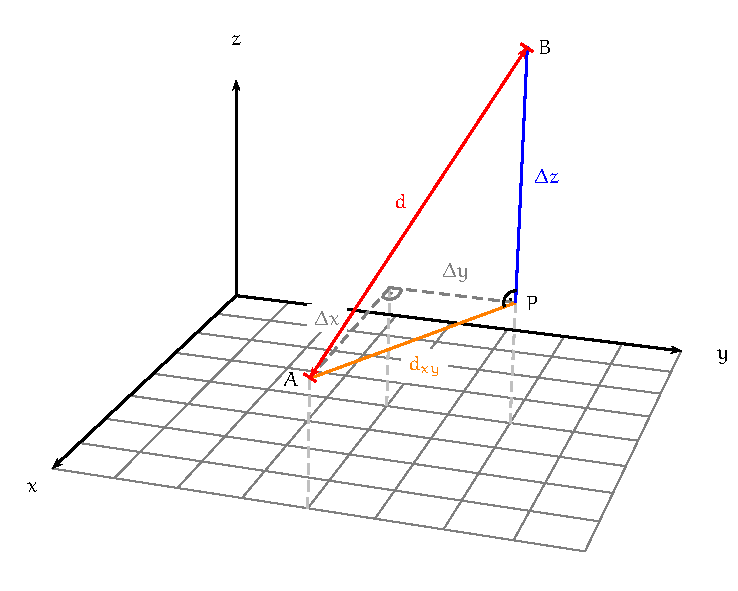
\includegraphics[width=\textwidth]{./distanz.pdf}
% distanz.pdf: 0x0 pixel, 300dpi, 0.00x0.00 cm, bb=
\caption{Abstand zweier Punkte im Raum}
\end{figure}
\end{folg}



\subsection{Berechnungen an Körpern}

\begin{folg}[Diagonale im Würfel]
 
\end{folg}

\begin{folg}[Diagonale im Quader]
 
\end{folg}

\begin{folg}[Höhe eines Tetraeders]
 
\end{folg}

\begin{folg}[Höhe einer Pyramide]
 
\end{folg}

\begin{folg}[Seitenhöhe einer Pyramide]
 
\end{folg}


\section{Trigonometrische Beziehungen}

\begin{figure}\begin{center}
                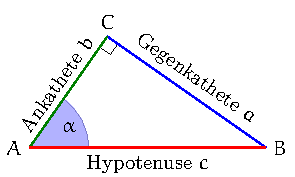
\includegraphics[width=.6\textwidth]{./rechtwinkliges_dreieck.pdf}
% rechtwinkliges_dreieck.pdf: 0x0 pixel, 300dpi, 0.00x0.00 cm, bb=

                \end{center}
\caption{Rechtwinkliges Dreieck}
\end{figure}

Die trigonometrischen Beziehungen Sinus, Kosinus und Tangens stellen einen Zusammenhang zwischen den Winkeln eines rechtwinkligen Dreiecks und den Verhältnissen der Seitenlängen her.

\begin{defi}[Sinus]
 Der \emph{Sinus} eines Winkels \(\alpha\) bezeichnet das Verhältnis der Streckenlänge von Gegenkathete \(a\) zu Hypotenuse \(c\) in einem rechtwinkligen Dreieck \(\triangle ABC\).
 \begin{equation*}
  \sin (\alpha ) = \frac{a}{c}
 \end{equation*}

\end{defi}

\begin{defi}[Kosinus]
 Der \emph{Kosinus} eines Winkels \(\alpha\) bezeichnet das Verhältnis der Streckenlänge von Ankathete \(b\) zu Hypotenuse \(c\) in einem rechtwinkligen Dreieck \(\triangle ABC\).
 \begin{equation*}
  \cos (\alpha ) = \frac{b}{c}
 \end{equation*}

\end{defi}

\begin{folg}
 Bei \(\alpha\) und \(\beta\) im rechtwinkligen Dreieck \(\triangle ABC\) sind die Werte von Sinus und Kosinus vertauscht.
 \begin{align*}
  \sin ( \alpha ) &= \cos(\beta)\\
  \cos (\alpha) &= \sin (\beta)
 \end{align*}

\end{folg}


\begin{defi}[Tangens]
 Der \emph{Tangens} eines Winkels \(\alpha\) bezeichnet das Verhältnis der Streckenlänge von Gegenkathete \(a\) zu Ankathete \(b\) in einem rechtwinkligen Dreieck \(\triangle ABC\).
 \begin{equation*}
  \tan (\alpha ) = \frac{a}{b}
 \end{equation*}
\end{defi}

\begin{folg}
 Der Tangens entspricht dem Verhältnis von Sinus zu Kosinus.
 \begin{align*}
  \tan (\alpha ) &= \frac{a}{b} = \frac{\frac{a}{c}}{\frac{b}{c}} = \frac{\sin(\alpha)}{\cos(\alpha)}\\
 \end{align*}

\end{folg}

\begin{beme}[Notation]
 Wenn aus dem Zusammenhang hervorgeht, was alles zum Argument von Sinus, Kosinus oder Tangens gehört, kann man auch die Klammern weglassen.
 \begin{align*}
  \cos \alpha &= \cos (\alpha) & \sin \alpha &= \sin (\alpha) & \tan \alpha &= \tan (\alpha)
 \end{align*}
Beachte: Die alleinige Angabe eines Ausdrucks wie \(\sin\) ist die Angabe einer Funktion, nicht die Angabe einer Zahl.
\end{beme}

\begin{regel}[Trigonometrie am Einheitskreis]
 \begin{figure}
\centering
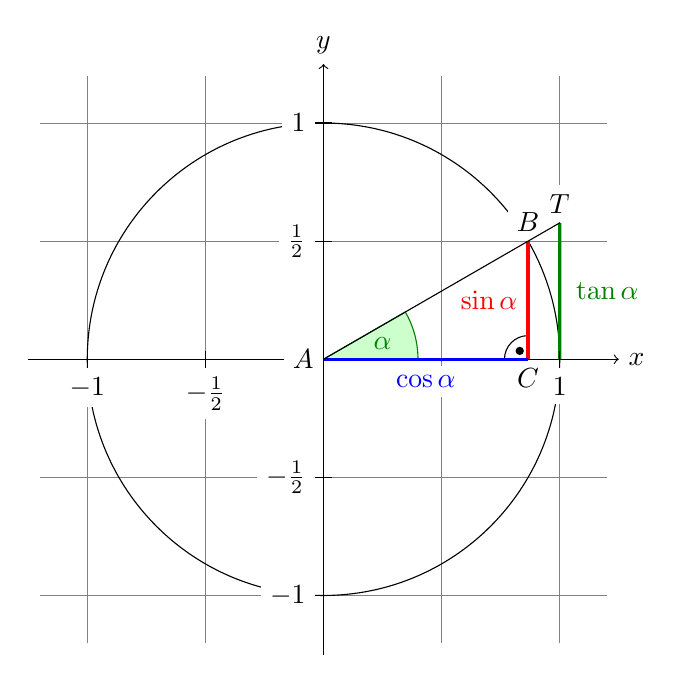
\begin{tikzpicture}[scale=3]
 \draw[step=.5cm, gray, very thin] (-1.2,-1.2) grid (1.2,1.2); 
 \filldraw[fill=green!20,draw=green!50!black] (0,0) -- (4mm,0mm) arc (0:30:4mm) -- cycle;
 \draw[green!50!black] (0.25,0) node[anchor=south] {\(\alpha\)};
 \draw[->] (-1.25,0) -- (1.25,0) coordinate (x axis) node[right] {$x$};
 \draw[->] (0,-1.25) -- (0,1.25) coordinate (y axis) node[above] {$y$};;
 \draw (0,0) circle (1cm);
 \coordinate (O) at (0,0);
 \coordinate (W) at (30:2cm);
 \coordinate (A) at (1,0);
 \coordinate (Z) at (1,1);
 \coordinate (T) at (intersection of O--W and A--Z);
 \coordinate (C) at (30:1cm |- x axis);
%  \draw (O) node[fill=white, anchor=north east]{0};
 \draw (O) node[fill=white, anchor= east]{\(A\)};
 \draw (30:1cm) node[fill=white, anchor=south]{\(B\)};
 \draw (C) -- +(-1mm,0mm) arc(180:90:1mm) -- cycle;
 \fill (C) +(135:0.5mm) circle (.5pt);
 \draw (C) node[fill=white, anchor=north]{\(C\)};
 \draw[very thick,red] (30:1cm) -- node[left,fill=white] {$\sin \alpha$} (30:1cm |- x axis);
 \draw[very thick,blue] (30:1cm |- x axis) -- node[below=2pt,fill=white] {$\cos \alpha$} (0,0);
 \draw[very thick,green!50!black] (1,0) --node[right=2pt,fill=white ] {$\tan \alpha$} (T);
 \draw (0,0) -- (T) node[fill=white, anchor=south]{\(T\)};
 \foreach \x/\xtext in {-1, -0.5/-\frac{1}{2}, 1} 
   \draw (\x cm,1pt) -- (\x cm,-1pt) node[anchor=north,fill=white] {$\xtext$};
 \foreach \y/\ytext in {-1, -0.5/-\frac{1}{2}, 0.5/\frac{1}{2}, 1} 
   \draw (1pt,\y cm) -- (-1pt,\y cm) node[anchor=east,fill=white] {$\ytext$};
 \end{tikzpicture}
 \caption{Die trigonometrischen Beziehungen am Einheitskreis}
\end{figure}
Der \emph{Einheitskreis} ist der Kreis mit Radius 1.

Trägt man den Winkel \(\alpha\) von der \(x\)-Achse aus an, so schneidet der zweite Schenkel des Winkels den Einheitskreis im Punkt \(B\). Der Lotfußpunkt durch \(B\) auf die \(x\)-Achse nennen wir \(C\). Gibt man dem Ursprung des Koordinatensystems noch die Bezeichnung \(A\), so ist das Dreieck \(\triangle ABC\) ein rechtwinkliges, dessen Hypotenuse die Länge 1 hat.

In einem Dreieck, dessen Hypotenusenlänge 1 beträgt, entsprechen die Längen der Katheten gerade dem Sinus und Kosinus des Winkels \(\alpha\).

\end{regel}


\begin{beme}[Trigonometrische Funktionen]
 Sinus, Kosinus und Tangens sind \emph{Funktionen}, die einen Winkel als Argument erwarten. Sie zeichnen sich durch einen charakteristischen Verlauf aus. Die Trigonometrischen Funktionen werden in der 10.~Jahrgangsstufe ausführlich behandelt.
 \begin{figure}
\centering
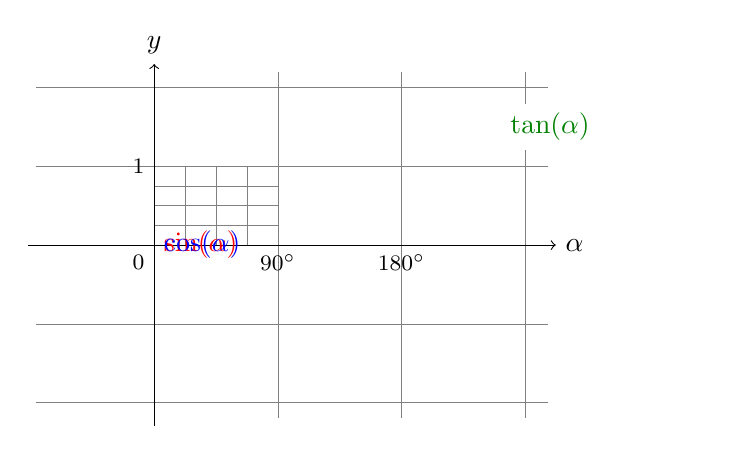
\begin{tikzpicture}[domain=-1.5:5,y=1cm,x=1cm,scale=1]
    \draw[very thin,color=gray, xstep=pi/2] (-1.5,-2.2) grid (5,2.2);
    \draw[very thin,color=gray, xstep=pi/8, ystep=0.25] (0,0) grid (pi/2,1);
    \draw[->] (-1.6,0) -- (5.1,0) node[right] {$\alpha$};
    \draw[->] (0,-2.3) -- (0,2.3) node[above] {$y$};
    \draw (0,0) node [anchor=north east] {\footnotesize \(0\)};
    \draw (pi/2,0) node [anchor=north] {\footnotesize  \(90^\circ\)};
    \draw (pi,0) node [anchor=north] {\footnotesize  \(180^\circ\)};
    \draw (0,1) node [anchor=east] {\footnotesize \(1\)};
    \clip (-1.6,-2.3) rectangle (7.1,2.3);
    \draw[color=red] plot[id=sinx, samples=200] function{sin(x)} node[right] {$\sin(\alpha)$};
%     \draw[color=red] node[right] {$f(x) =\sin(x)$};
%     \draw[color=red] (4,16) circle (2pt) node[anchor=west] {\((4|16)\)};
    \draw[color=blue] plot[id=cosx, samples=200] function{cos(x)} 
        node[right] {$\cos(\alpha)$};
    \draw[color=green!50!black] plot[id=tanx, domain=(-pi/2+0.1):(pi/2-0.1), samples=200] function{tan(x)}; 
    \draw[color=green!50!black] plot[id=tan2x,  domain=(pi/2+0.1):(3*pi/2-0.1), samples=200] function{tan(x)};
    \draw[color=green!50!black] (4.4,1.5) node[right,fill=white] {$\tan(\alpha)$};   
\end{tikzpicture}
\caption{Graphen trigonometrischer Funktionen}
\end{figure}
 
\end{beme}



\begin{defi}[Umkehrungen der trig. Funktionen]
 
\end{defi}


\begin{beme}[Potenzen trigonometrischer Funktionen]
 
\end{beme}


\begin{ssatz}
 Die Summe der Quadrate von Sinus und Kosinus des gleichen Winkels ergibt immer den Wert \(1\).
 
 \begin{blockwhitebox}
  \begin{equation*}
   \sin^2 \alpha + \cos^2 \alpha = 1 
  \end{equation*}

 \end{blockwhitebox}

\end{ssatz}

\section{Prisma, Pyramide, Zylinder \& Kegel}

\begin{defi}[Prisma]Ein \emph{Prisma} ist ein Körper, der ein Vieleck -- ein sogenannetes \emph{Polygon} -- als Grundfläche besitzt und dessen Boden und Decke parallel zueinander liegen.
 
Man unterscheidet ein \emph{gerades Prisma}, bei dem die Seitenflächen senkrecht auf der Grundfläche stehen, von einem \emph{schiefen Prisma}.
\begin{figure}
  \begin{center}
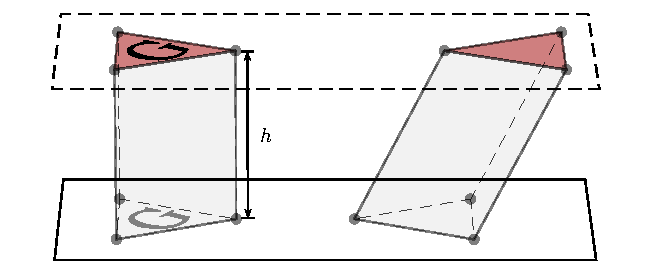
\includegraphics[height=4cm]{./prisma.pdf}
% prisma.pdf: 0x0 pixel, 300dpi, 0.00x0.00 cm, bb=
\caption{Gerades und schiefes Prisma}
\end{center}
 \end{figure}

\end{defi}

\begin{regel}[Volumen des Prismas]
 Für jedes Prisma gilt:
 \begin{equation*}
  V = G \cdot h
 \end{equation*}
 Das Volumen ist das Produkt aus Grundfläche und Höhe.
\end{regel}

\begin{regel}[Prinzip von \textsc{Cavalieri}]
 Haben die Querschnittsflächen zwei Körper in jeder Höhe den gleichen Flächeninhalt und haben sie die gleiche Höhe, so ist ihr Volumen gleich.
 \begin{figure}
  \begin{center}
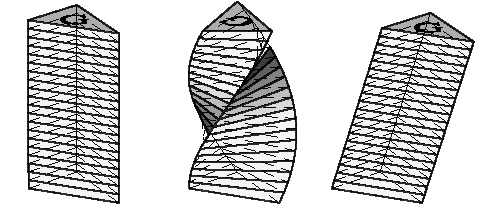
\includegraphics[height=4cm]{./prisma2.pdf}
% prisma.pdf: 0x0 pixel, 300dpi, 0.00x0.00 cm, bb=
\caption{Körper mit gleichen Querschnittsflächen}
\end{center}
 \end{figure}
 
 Also egal, wie die eine Querschnittsfläche gegenüber der Grundfläche verschoben, gedreht oder in Teile zerteilt wird, das Volumen des Körpers bleibt gleich.
\end{regel}

\begin{regel}[Oberfläche des Prismas]
 Die Oberfläche eines Prismas besteht aus dem Doppelten der Grundfläche \(G\) (Boden und Deckel) und der \emph{Mantelfläche} \(M\).
 \begin{equation*}
  O = 2\cdot G + M
 \end{equation*}
 Die Mantelfläche beim geraden Prisma besteht aus Rechtecken. Daher ist die Mantelfläche gleich der Summe aus den Produkten der Höhe mit den Seitenlägen der Grundfläche.
 \begin{equation*}
  M = a\cdot h + b\cdot h + \ldots
 \end{equation*}
\end{regel}

\begin{defi}[Zylinder]
 Ein \emph{Zylinder} ist ein Körper, dessen Boden und Decke -- genauso wie beim Prisma -- parallel zueinander liegen und gleich groß sind. Die Grundfläche bildet jedoch ein Kreis und die \emph{Mantelfläche} ist gekrümmt.
 \begin{figure}
  \begin{center}
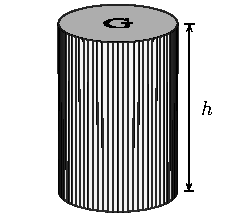
\includegraphics[height=4cm]{./zylinder.pdf}
% prisma.pdf: 0x0 pixel, 300dpi, 0.00x0.00 cm, bb=
\caption{Zylinder}
\end{center}
 \end{figure}
\end{defi}

\begin{regel}[Volumen des Zylinders]
 Das Volumen eines Zylinders berechnet man über das Produkt von Flächeninhalt der Grundfläche~\(G\) mit der Höhe~\(h\) des Zylinders.
 \begin{equation*}
  V_{\text{Zyl}} = G\cdot h = r^2\pi \cdot h
 \end{equation*}
\end{regel}

\begin{regel}[Oberfläche des Zylinders]
 Die Oberfläche eines Zylinders setzt aus den Flächeninhalten der Grund- und Deckfläche~\(G\), sowie der Mantelfläche~\(M\) zusammen. Es gilt:
 \begin{align*}
  M &= 2\pi r \cdot h \\
  O_{\text{Zyl}} &= 2G + M = 2 r^2 \pi +  2\pi r \cdot h = 2\pi r\cdot ( r+h)
 \end{align*}

\end{regel}

\begin{defi}[Pyramide]
 Eine \emph{Pyramide} ist ein Körper, der ein Vieleck als Grundfläche besitzt und von den Eckpunkten der Grundfläche sich alle restlichen Kanten in einem Punkt -- der Spitze -- treffen.
\end{defi}

\begin{regel}[Netz einer Pyramide]
 
\end{regel}


\begin{regel}[Volumen der Pyramide]
 
\end{regel}

\begin{defi}[Kegel]
 
\end{defi}

\begin{regel}[Netz eines Kegels]
 
\end{regel}


\begin{regel}[Volumen des Kegels]
 
\end{regel}


\chapter{Stochastik der 9.~Jahrgangsstufe}

\epigraph{Gott existiert oder nicht. Entweder ich glaube an Gott oder nicht. Von diesen vier Möglichkeiten ist nur eine zu meinem Nachteil. Damit ich diese vermeide, glaube ich an Gott.}{\textsc{Blaise Pascal}}

\section{Zusammengesetzte Zufallsexperimente}
Baumdiagramm, Urnenmodell

\section{Pfadregeln}